\ProvidesFile{ch3.tex}[Chapter3]
\chapter{QUANTUM ENHANCED LOCALIZATION MICROSCOPY WITH A SINGLE PHOTON AVALANCHE DIODE ARRAY}
\ix{physics//Physics appendix}

\section{Background}

\subsection{A brief introduction to quantum optics}

Experimental techniques have surfaced which take advantage of the quantum nature of light to enhance imaging methods. The advent of fast and sensitive detectors allows us to measure electromagnetic fields at a timescale where quantum effects can be seen. We often speak of methods such as photon counting or photon statistics, and it is prudent to briefly define the photon and how it can be measured with this technology.

Quantization of the electromagnetic field generally begins by writing a Fourier expansion of solutions to Maxwell's equations called \emph{modes} and identifying the canonical position and momentum variables. This procedure is out of the scope of this thesis. Instead, we start by stating the major result of quantization, in which each mode of the field is quantized as a quantum harmonic oscillator. As such, the Hamiltonian for one particular mode has energy eigenvalues $E_{k} = \hbar\omega_{k}(n + \frac{1}{2})$ for mode $k$ with frequency $\omega_{k}$. Since there may be infinitely many modes, the wavefunction is $\ket{\psi} = \ket{n_{1},n_{2},...}$ where $n_1$ is the number of photons in the first mode, $n_2$ is the number of photons in the second mode, and so on. The number operator for the $k$-th mode gives $\hat{n}_k\ket{\psi} = n_{k}\ket{\psi}$.

The number operator $\hat{n}_k = \hat{a}_k^\dagger\hat{a}_k$ is defined in terms of operators $\hat{a}_k$ and $\hat{a}_k^\dagger$ which are photon annihilation and creation operators for the $k$-th mode, respectively. These operators satisfy the commutation relations $[\hat{a}_k, \hat{a}_{k'}^\dagger] = \delta_{kk'}$ and $[\hat{a}_k, \hat{a}_{k'}] = [\hat{a}_k^\dagger, \hat{a}_k^\dagger] = 0$. The action of the annihilation and creation operators on the joint number states is:

\begin{equation*}
\hat{a}_k \ket{n_1, n_2, ...} = \sqrt{n_k} \ket{n_1, n_2, ...} \;\;
\hat{a}_k^\dagger \ket{n_1, n_2, ...} = \sqrt{n_k + 1} \ket{n_1, n_2, ...}
\end{equation*}

\subsection{Photon statistics}

\begin{figure*}[t]
\centering
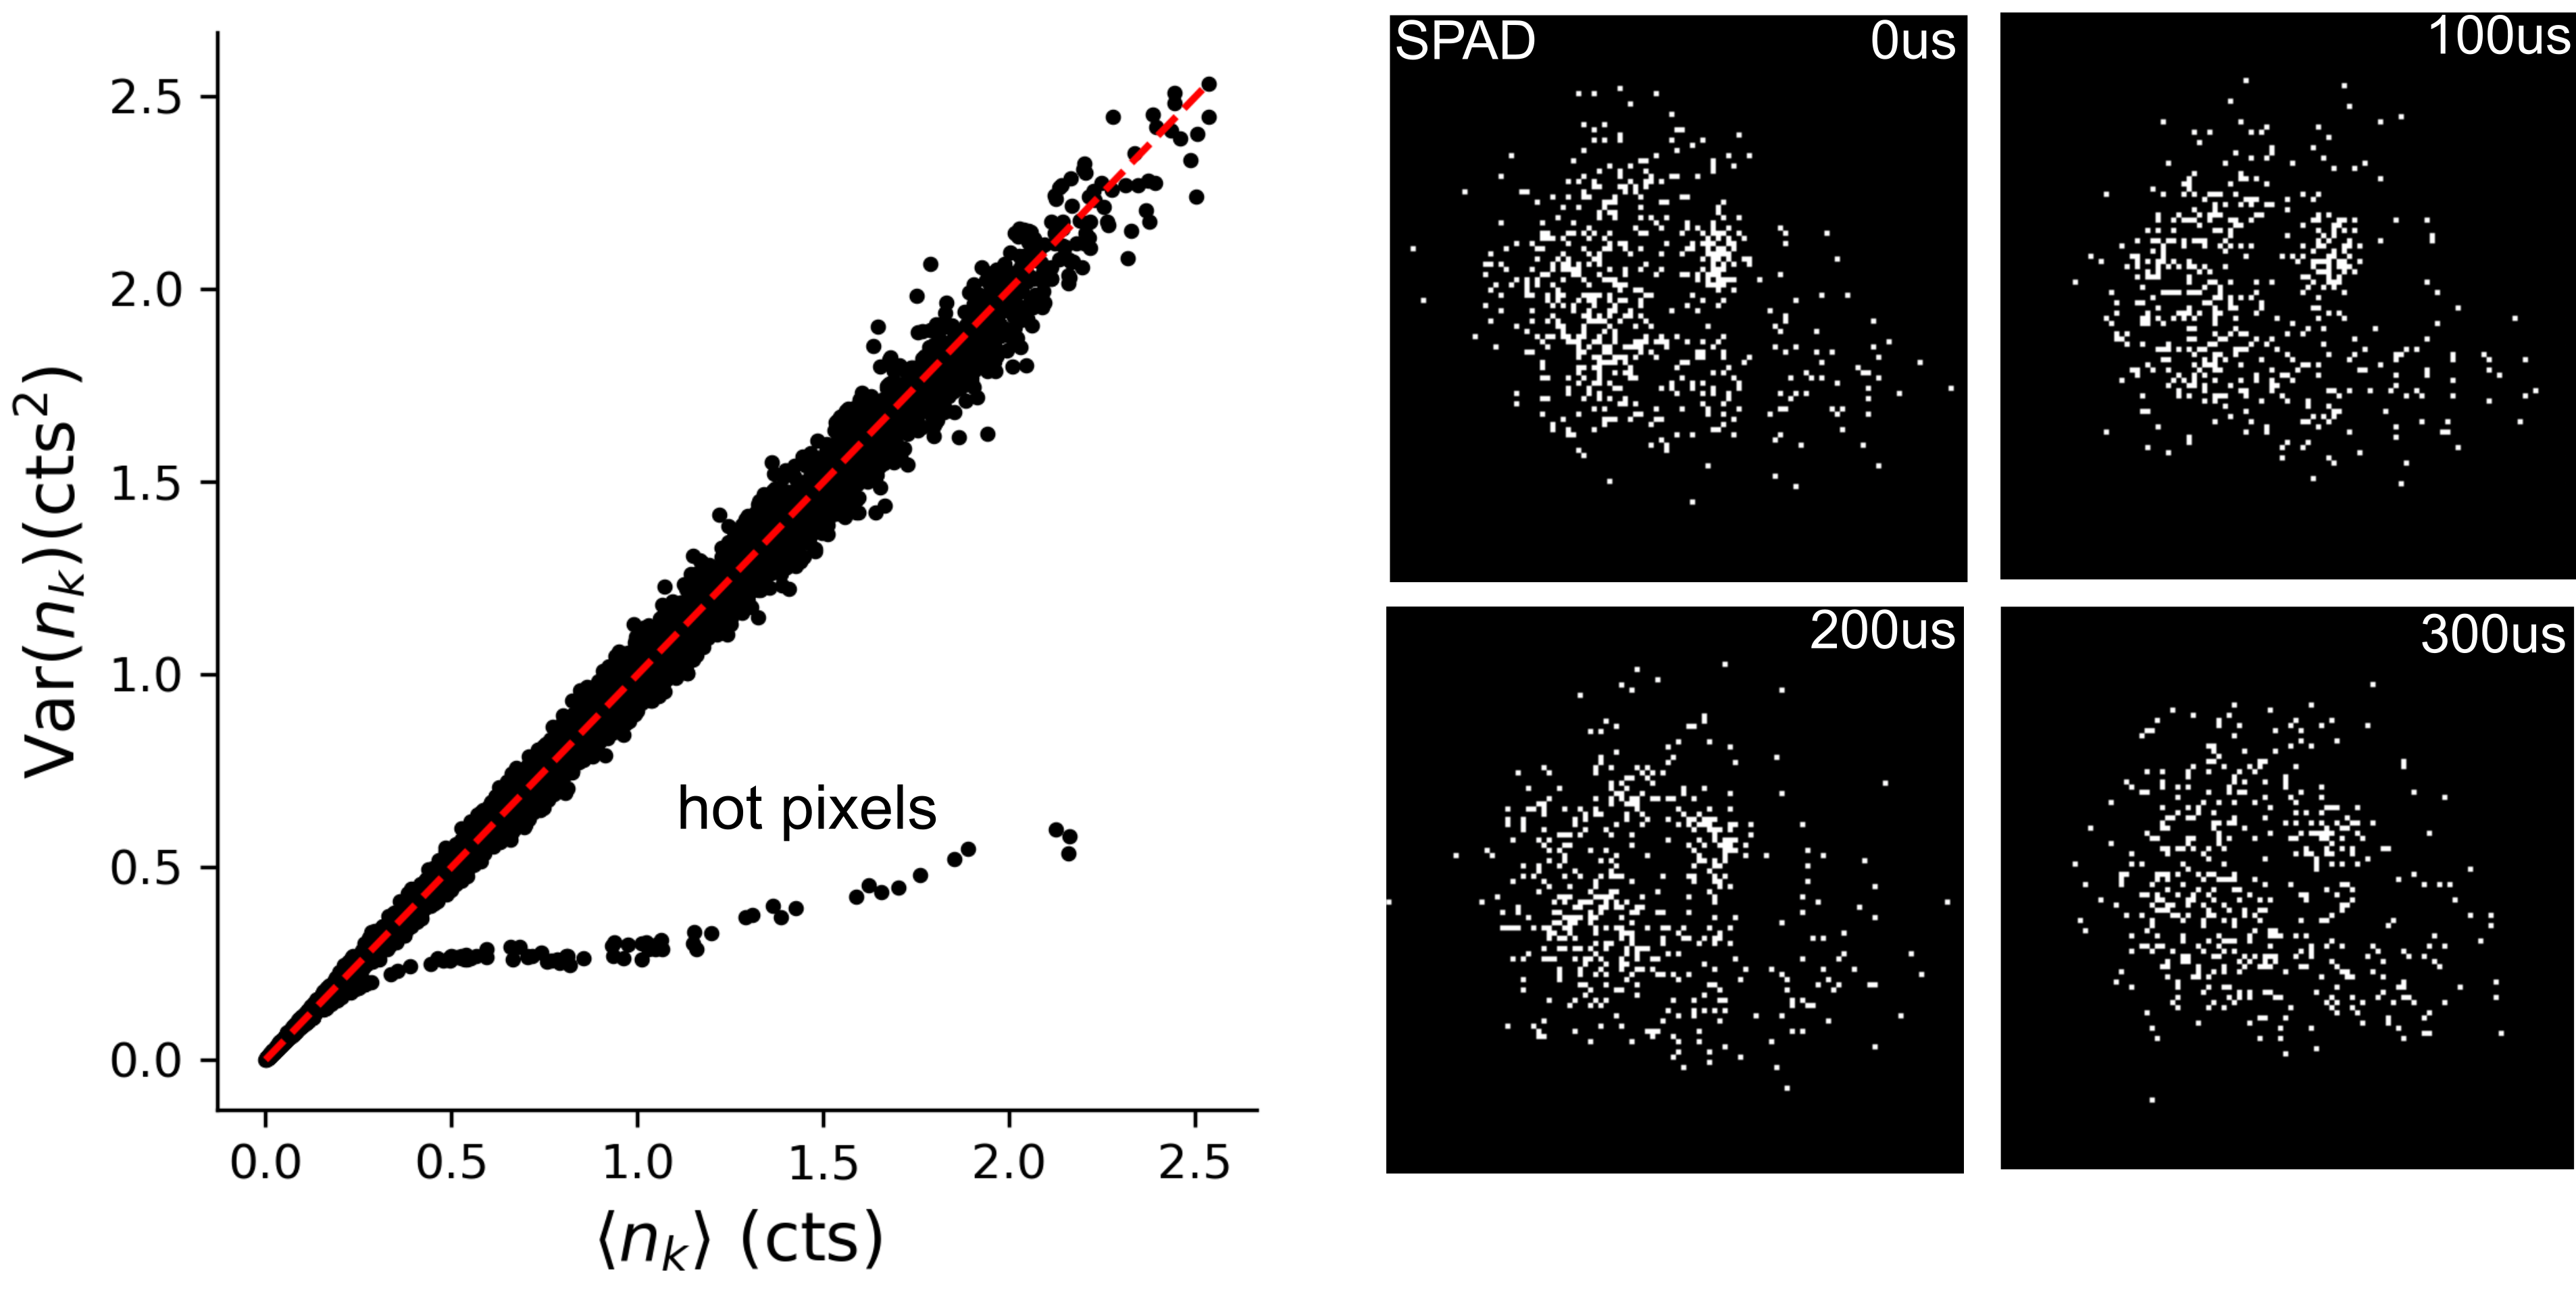
\includegraphics[width=16cm]{/Users/cwseitz/git/cwseitz.github.io/docs/phd/spad/spad/media/Laser-Stats.png}
\caption{\textbf{Poissonian photon statistics of a Gaussian laser spot} (left) Fano factor plot of pixel-wise variance in photon counts with respect to average photon counts, for 100us exposures of a Gaussian beam pulsed at 10MHz. Equal mean and variance (Poisson statistics) showed as a dashed red line. (right) Example images taken in sequence with the SPAD array.}
\label{fig:fig29}
\end{figure*}    

There are certain states $\ket{\psi}$ which have special properties, such as the coherent state. Coherent states resemble classical oscillations of the EM field. A coherent state $\ket{\alpha}$ is defined as the eigenstate of the annihilation operator $\hat{a}$:

\begin{equation*}
\hat{a} \ket{\alpha} = \alpha \ket{\alpha}
\end{equation*}

where $\alpha$ is a complex number. The coherent state for a single mode field is given by:

\begin{equation*}
\ket{\alpha} = e^{-\frac{\lvert\alpha\lvert^2}{2}} \sum_{n=0}^\infty \frac{\alpha^n}{n!} \ket{n}
\end{equation*}

It turns out that if we measure a number of photons in this state, we would find that the number of photons has Poisson statistics. To see this, we calculate the probability $p(n)$ of finding $n$ photons in a coherent state $\ket{\alpha}$:

\begin{equation*}
p(n) = \lvert \bra{n} \ket{\alpha} \lvert^2 = \lvert e^{-\frac{\lvert\alpha\lvert^2}{2}} \frac{\alpha^n}{n!} \lvert^2 = e^{-\lvert\alpha\lvert^2} \frac{\lvert\alpha\lvert^{2n}}{n!}
\end{equation*}

This is simply the Poisson distribution with mean $\langle \hat{n} \rangle = \lvert\alpha\lvert^2$. The variance of the photon number distribution in a coherent state is also $\lvert\alpha\lvert^2$, characteristic of Poisson statistics, where the mean and variance are equal. Poissonian fluctuations of a Gaussian beam can be spatially resolved using a single photon avalanche diode (SPAD) array (Figure \ref{fig:fig29}).

In contrast, single photon states, such as $\ket{1}$, do not necessarily follow Poisson statistics. This state could be prepared by an isolated single photon source such as a fluorescent dye molecule, quantum dot, or nitrogen vacancy, which can produce only a single photon at at time. This phenomenon is referred to as \emph{fluorescence antibunching} where photons tend to be detected as isolated events rather than in bursts or bunches. Single photon sources have a fluorescence lifetime, typically on the order of nanoseconds, which results in a sequence of photon arrivals with a more regular structure than would be expected under Poisson statistics. Note that for such a single photon source the single-mode field can be in state $\ket{1}$ but not state $\ket{2}$ at any given time. If more single photon sources are present or multi-level relaxations occur, states beyond $\ket{1}$ are possible. This has led to the introduction of binomial states of the quantized field \parencite{Stoler1985}. This fact is leveraged in the following sections, to count the number of single photon sources in a region of interest using a SPAD array.

\section{Second-order coherence}

The second-order coherence function, $ g^{(2)}(\tau) $, is a fundamental tool in quantum optics, providing insight into photon statistics. It can be expressed in terms of photon counts $ n(t) $ as:

\begin{equation}
g^{(2)}(\tau) = \frac{\langle n(t) n(t+\tau) \rangle}{\langle n(t) \rangle^2}
\end{equation}

This formulation highlights how the intensity correlations between photons detected at times $ t $ and $ t+\tau $ are normalized by the square of the mean photon count rate, providing a dimensionless measure of the correlation. The value of $ g^{(2)}(\tau) $ and its dependence on $ \tau $ reveal essential characteristics of the light source. For sub-Poissonian statistics, which is synonymous with photon antibunching, $ g^{(2)}(0) < 1$ and the likelihood of detecting two photons in quick succession is reduced. This behavior is closely related to the fluorescence lifetime of the emitters; after emitting a photon, a fluorophore requires a characteristic time to re-enter the excited state, leading to a dip in $ g^{(2)}(\tau) $ at short $ \tau $. Coherent light, discussed in the previous section, shows no correlation between photon arrival times, resulting in $ g^{(2)}(\tau) = 1 $ for all $ \tau $. Super-Poissonian statistics, seen in thermal light, exhibit photon bunching, where $ g^{(2)}(\tau) $ starts high at $ \tau = 0 $ and decays to 1 as $ \tau $ increases, indicating a higher probability of photons arriving close together in time.

Techniques such as Hanbury Brown and Twiss (HBT) interferometry are commonly employed to measure $ g^{(2)}(\tau) $, using two single photon sensitive detectors and a beam splitter. In the following sections, we will incorporate an empirical estimate of $g^{(2)}(\tau)$ into a framework for inference of the number of fluorescent emitters in a diffraction limited region. 

\section{Quantum-enhanced localization microscopy}

Single photon avalanche diodes (SPADs) have long been the detector of choice for highly sensitive biological imaging and sensing, such as single molecule imaging and single molecule spectroscopy. Its fast temporal response and low background noise allow for the registration of a single photon with a temporal resolution as precise as several picoseconds \parencite{Bruschini2019}. However, standard SPAD detectors lack spatial resolution and are typically integrated in laser scanning microscopes for biological imaging, which significantly limits the imaging speed. Recently developed SPAD arrays removed this limitation and extended the high spatiotemporal imaging to widefield microscopy. SPAD arrays can achieve orders of magnitude higher temporal resolutions than standard cameras while preserving the SPAD detector‘s original signatures, such as single photon sensitivity, low dark count rates, and time-gated photon collection. Furthermore, the reduced readout noise and large fill-factor of recently commercialized SPAD arrays suggests their use for precision widefield bioimaging for single molecule studies. Such technologies have also attracted considerable attention in the bioimaging community for various applications including widefield fluorescence lifetime imaging \parencite{Nedbal2024,Ulku2019,Zickus2020}.

The spatial configuration of the SPAD array can also function as a two-dimensional and on-chip Hanbury-Brown and Twiss setup that measures the antibunching effect, which is a purely quantum optical phenomenon \parencite{Tenne2019,Treussart2001,Schwartz2012,Ta2010} that reports the single photon emission signature of a quantum emitter. A simplified SPAD array has been previously discussed for localization microscopy in non-sparse scenes \parencite{Israel2017} to image quantum dots beyond the diffraction limit. However, this imaging modality was challenged by a general issue encountered in fluorescent labeling, i.e., how to quantify multiple fluorophores in a diffraction-limited spot? 

The antibunching property is manifest in both the second-order coherence of photon arrivals as well as the photon counting histogram (PCH) \parencite{Chen1999,Huang2004} i.e., the distribution of the number of photons collected from a diffraction-limited volume. Importantly, the number of photons detected during high-speed imaging provides evidence for the number of single photon sources present in the imaged region. Previous studies have used the PCH to quantify the number of active fluorescent emitters by using conventional SPAD detectors in confocal setups. However, using a SPAD array, the PCH can be measured over a large field of view with spatial resolution by fast acquisition of binary images synchronized with pulsed laser excitation. 

Here, we demonstrate that the PCH can be parameterized by the number of active fluorescent emitters in a region of interest (ROI) and their associated molecular brightness. Then, by integrating the PCH into a Bayesian inference scheme, the relative probability of various numbers of fluorescent emitters can be compared, while expressing uncertainty in the molecular brightness. We experimentally demonstrate the model by counting quantum dots and varying numbers of fluorescent dye molecules attached to DNA origamis. In parallel, we theoretically examine second-order coherence of single-molecule fluorescence as a validation metric in both background-free environments and in the presence of a coherent background signal. Our findings indicate that sensitivity of the second order coherence to background conditions limits its effectiveness to scenarios with high signal-to-background ratios.

%Far-field optical microscopy is fundamentally limited by diffraction, with the maximum attainable resolution being limited to approximately half the wavelength of light. Several schemes to beat the diffraction limit have been developed in recent years. Many of these schemes utilize the concept of precise localization of isolated fluorescent emitters which blink over a time series of frames \parencite{Rust2006,Betzig2006}. An inherent problem with such methods is the requirement that fluorescent emitters be isolated, slowing down the acquisition of super-resolved images. To begin to address this issue, we leverage the fact that many fluorophores are intrinsically single photon sources and exhibit fluorescence antibunching. This property can constrain the number of active fluorescent emitters in a region of interest (ROI) and can potentially enable localization in non-sparse scenes \parencite{Ta2010,Israel2017}. 

%\begin{figure*}[t]
%\centering
%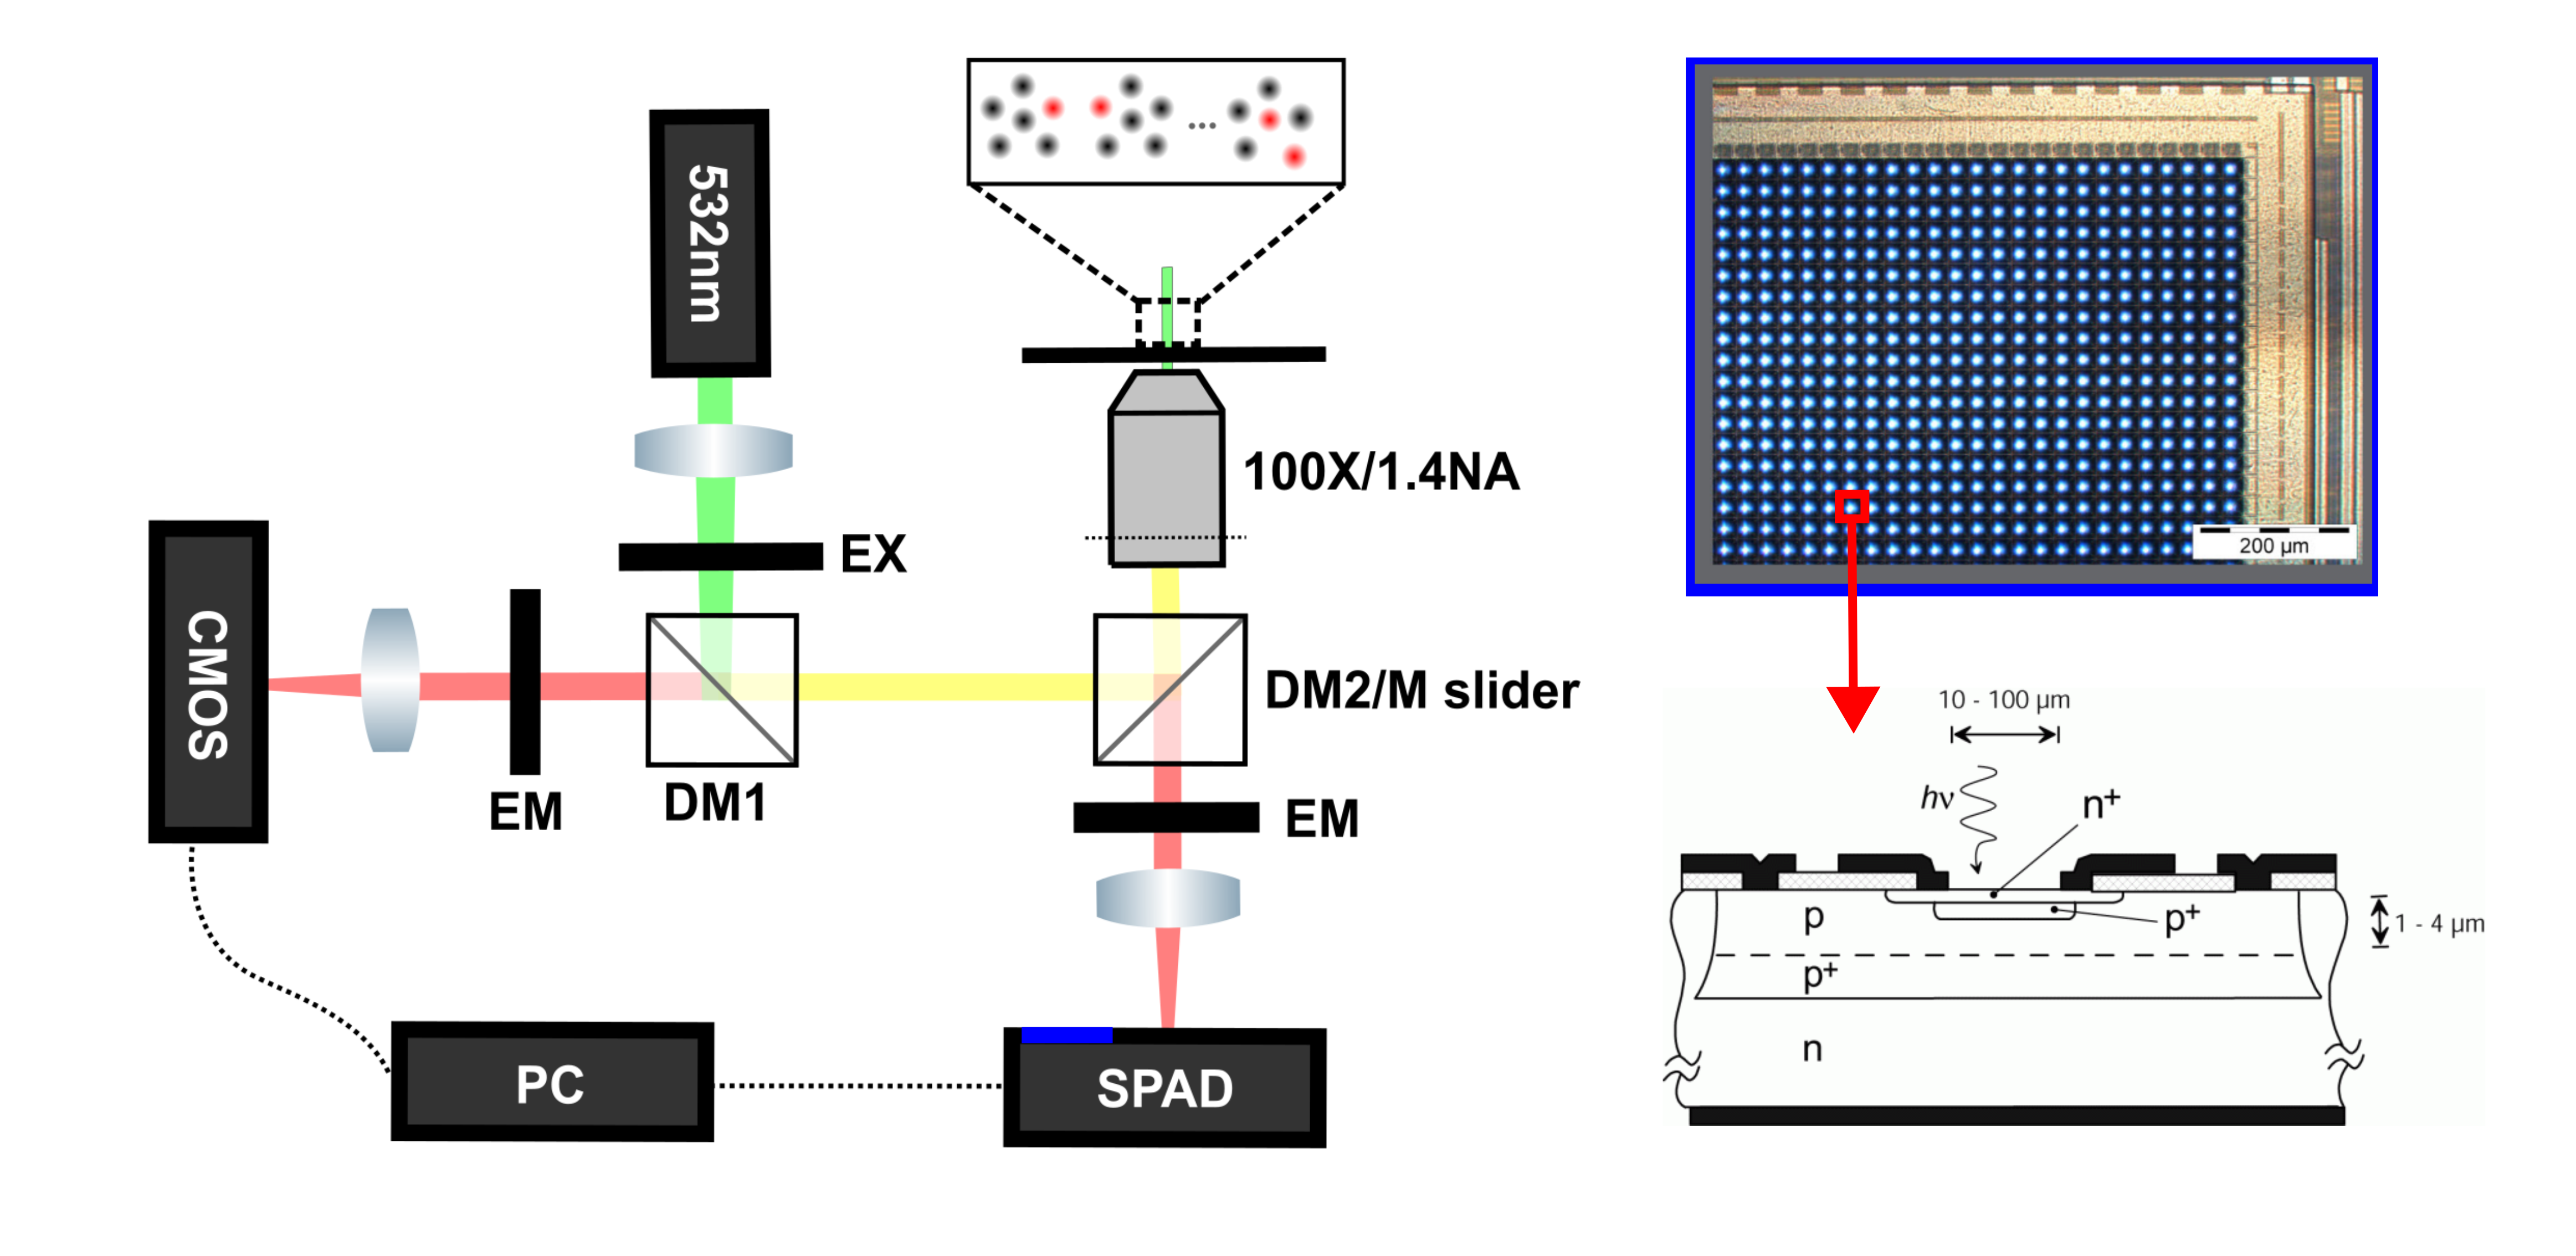
\includegraphics[width=15cm]{/Users/cwseitz/git/cwseitz.github.io/docs/phd/spad/spad/media/SPADD.png}
%\caption{\textbf{Experimental setup for widefield photon counting}. (left) A 532nm pulsed laser is directed through filtering and focusing optics to a 100X oil-immersion objective. Emisson light is collected by a CMOS or SPAD sensor. (right) Diagram of the diode at each pixel of the SPAD array. Sensor micrograph courtesy of Pi Imaging Technologies}
%\label{fig:fig00}
%\end{figure*}    

%\begin{figure*}[t]
%\centering
%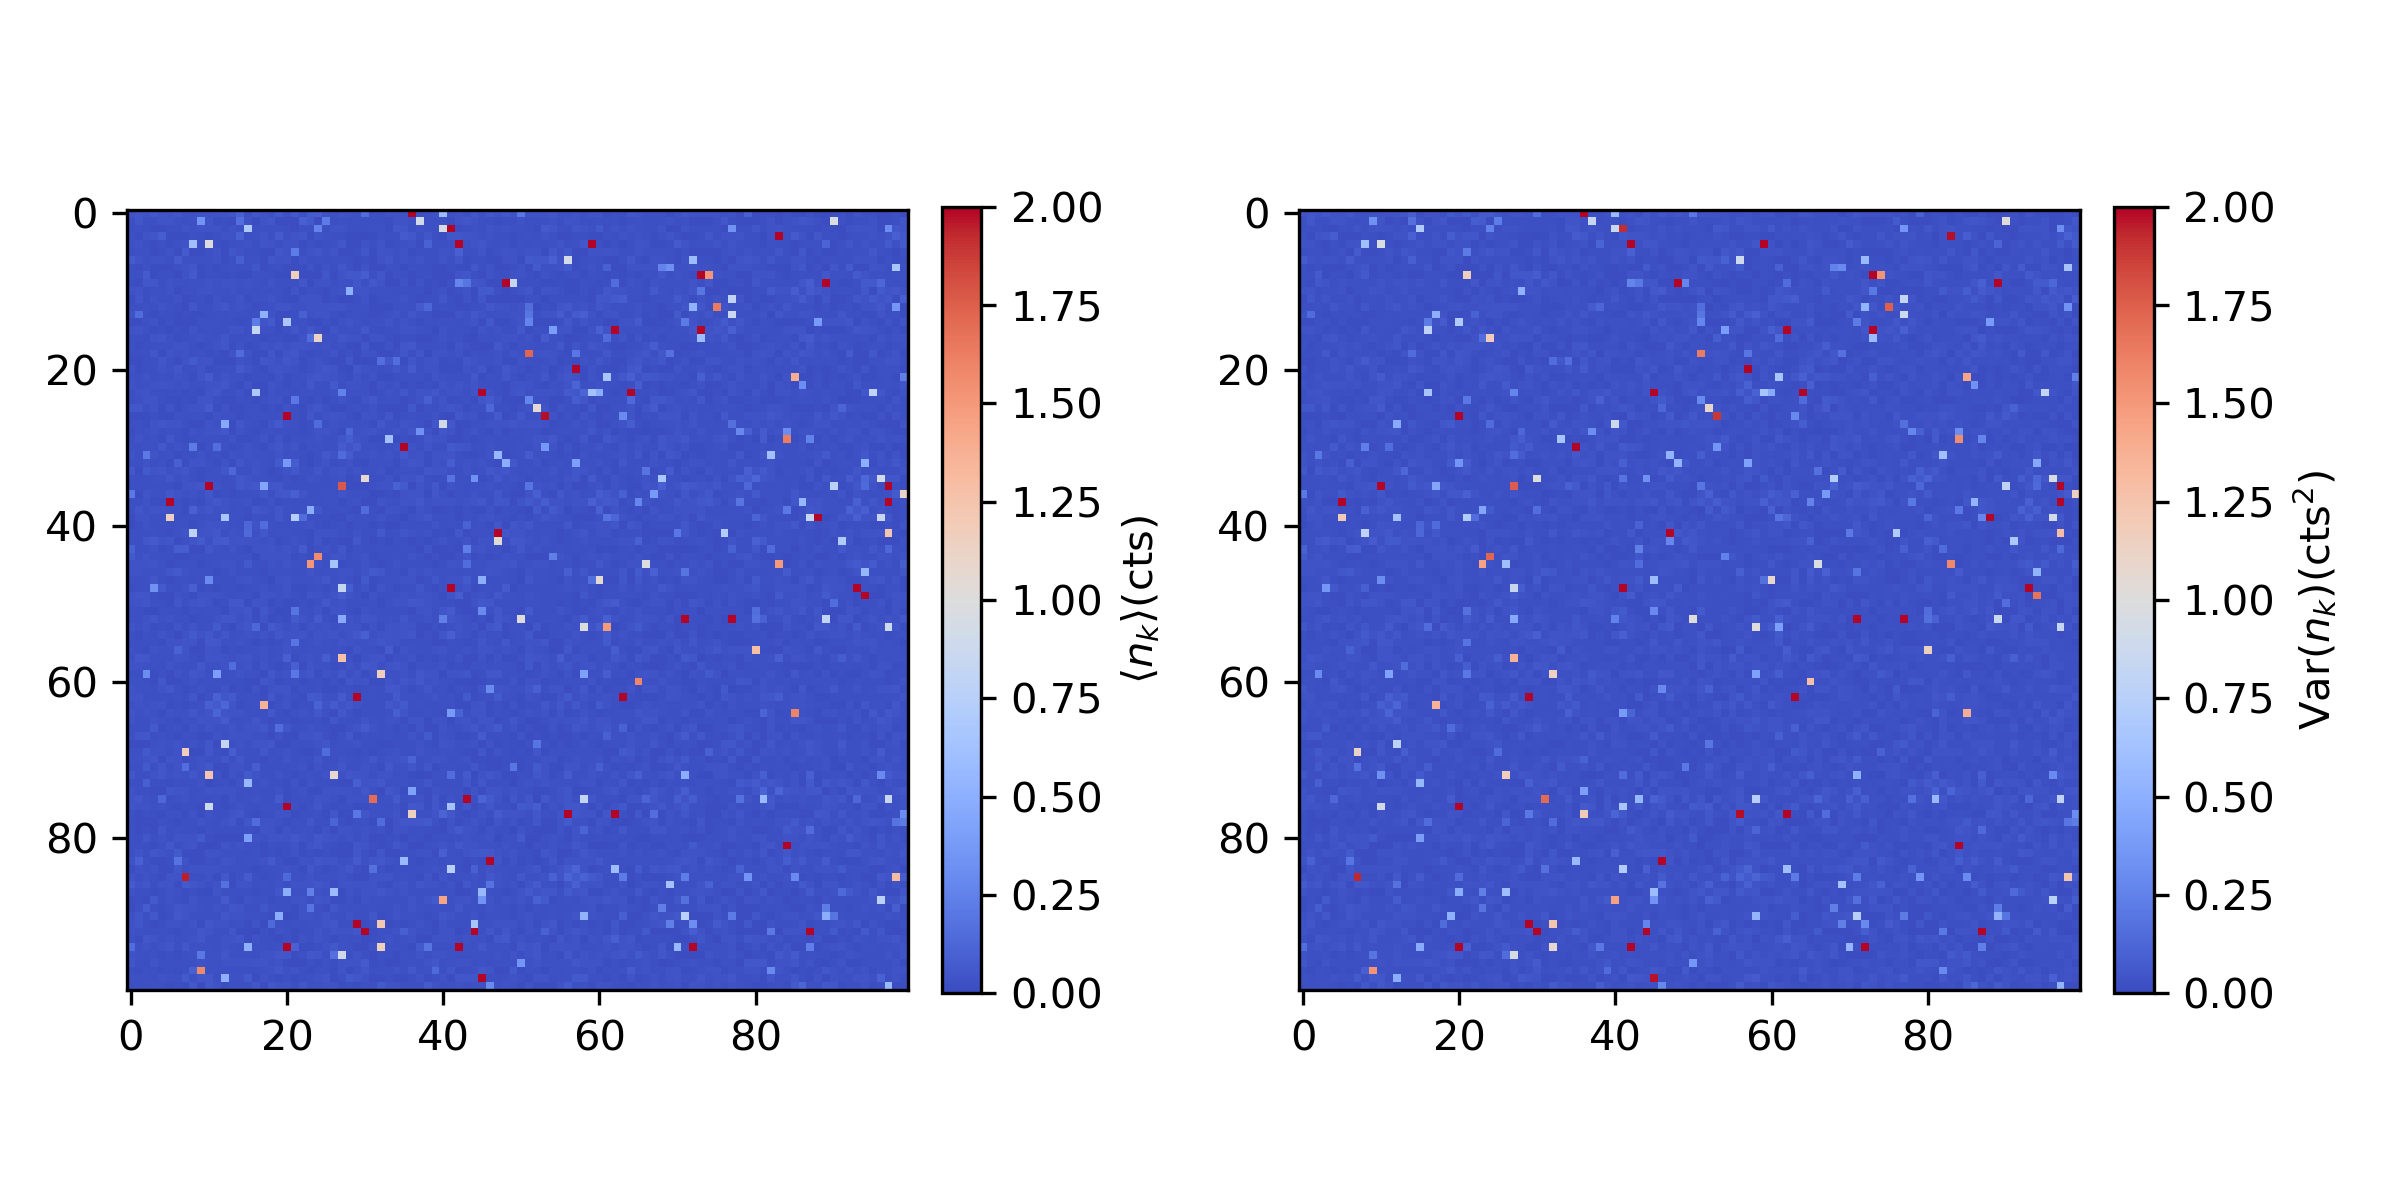
\includegraphics[width=14cm]{/Users/cwseitz/git/cwseitz.github.io/docs/phd/spad/spad/media/Dark.png}
%\caption{\textbf{Dark counts of the SPAD array}. (left) Average pixel-wise dark counts for a 100x100 pixel region exposed for 100ms (right) Variance of dark counts for 100ms exposure.}
%\label{fig:fig30}
%\end{figure*}


\begin{figure*}[t]
\centering
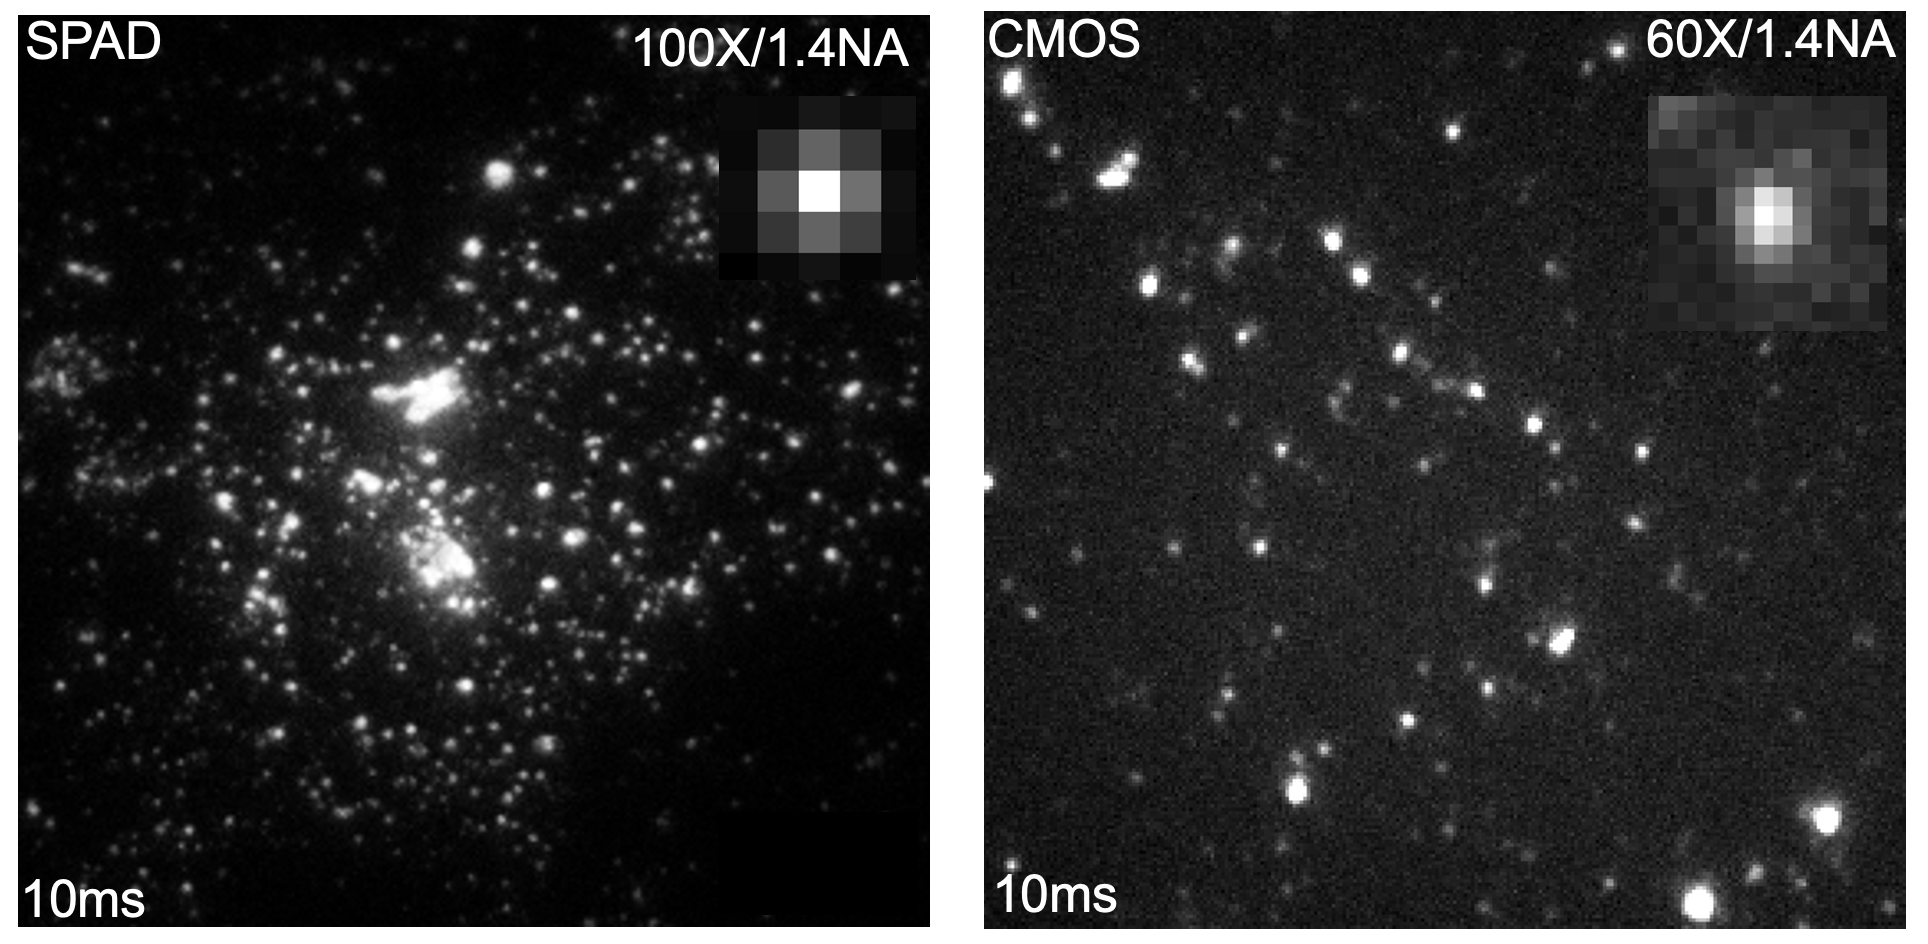
\includegraphics[width=14cm]{/Users/cwseitz/git/cwseitz.github.io/docs/phd/spad/spad/media/SPADvCMOS.png}
\caption{\textbf{Comparison of quantum dot images between CMOS and SPAD cameras} (left) SPAD image of Qdot655 coated on a glass coverslip using a 100X/1.4NA oil-immersion objective and a 10ms exposure time (right) CMOS image of Qdot655 using a 60X/1.4NA oil-immersion objective and a 10ms exposure time. Both use continuous-wave 640nm excitation}
\label{fig:fig4}
\end{figure*}    

%Molecular counting with fluorescence antibunching has a fairly simple motivation: coincidence of photons at multiple detector elements during high speed imaging provides evidence for the number of single photon sources present in the imaged region. Combining the ideas of conventional super-resolution approaches with photon statistics may prove to be a powerful set of methods for bioimaging. SPAD cameras achieve orders of magnitude higher temporal resolutions than standard CMOS cameras, single photon sensitivity, and dark count rates less than 25 counts per second (Figure \ref{fig:fig30}). Furthermore, the reduced readout noise and large fill-factor of recently commercialized SPAD arrays suggests their use for single molecule localization with reduced uncertainty.

%Here, we present a method for widefield single photon counting in order to count fluorophores in the sample and subsequently constrain single molecule localization. We investigate the theoretical properties of the zero-lag, second-order coherence function $g^{(2)}(0)$ for widefield photon counting and its spatial properties (Figure \ref{fig:fig5}). Using Bayesian analysis, we derive a posterior distribution on the number of active fluorescent emitters in a region of interest. This result is then combined with single molecule localization algorithms.  We demonstrate resolution of multiple emitters using a multi-emitter fitting algorithm and report localization errors with respect to the CRLB.


\subsection{Results}

\subsubsection{Model}

\begin{figure*}[t]
\centering
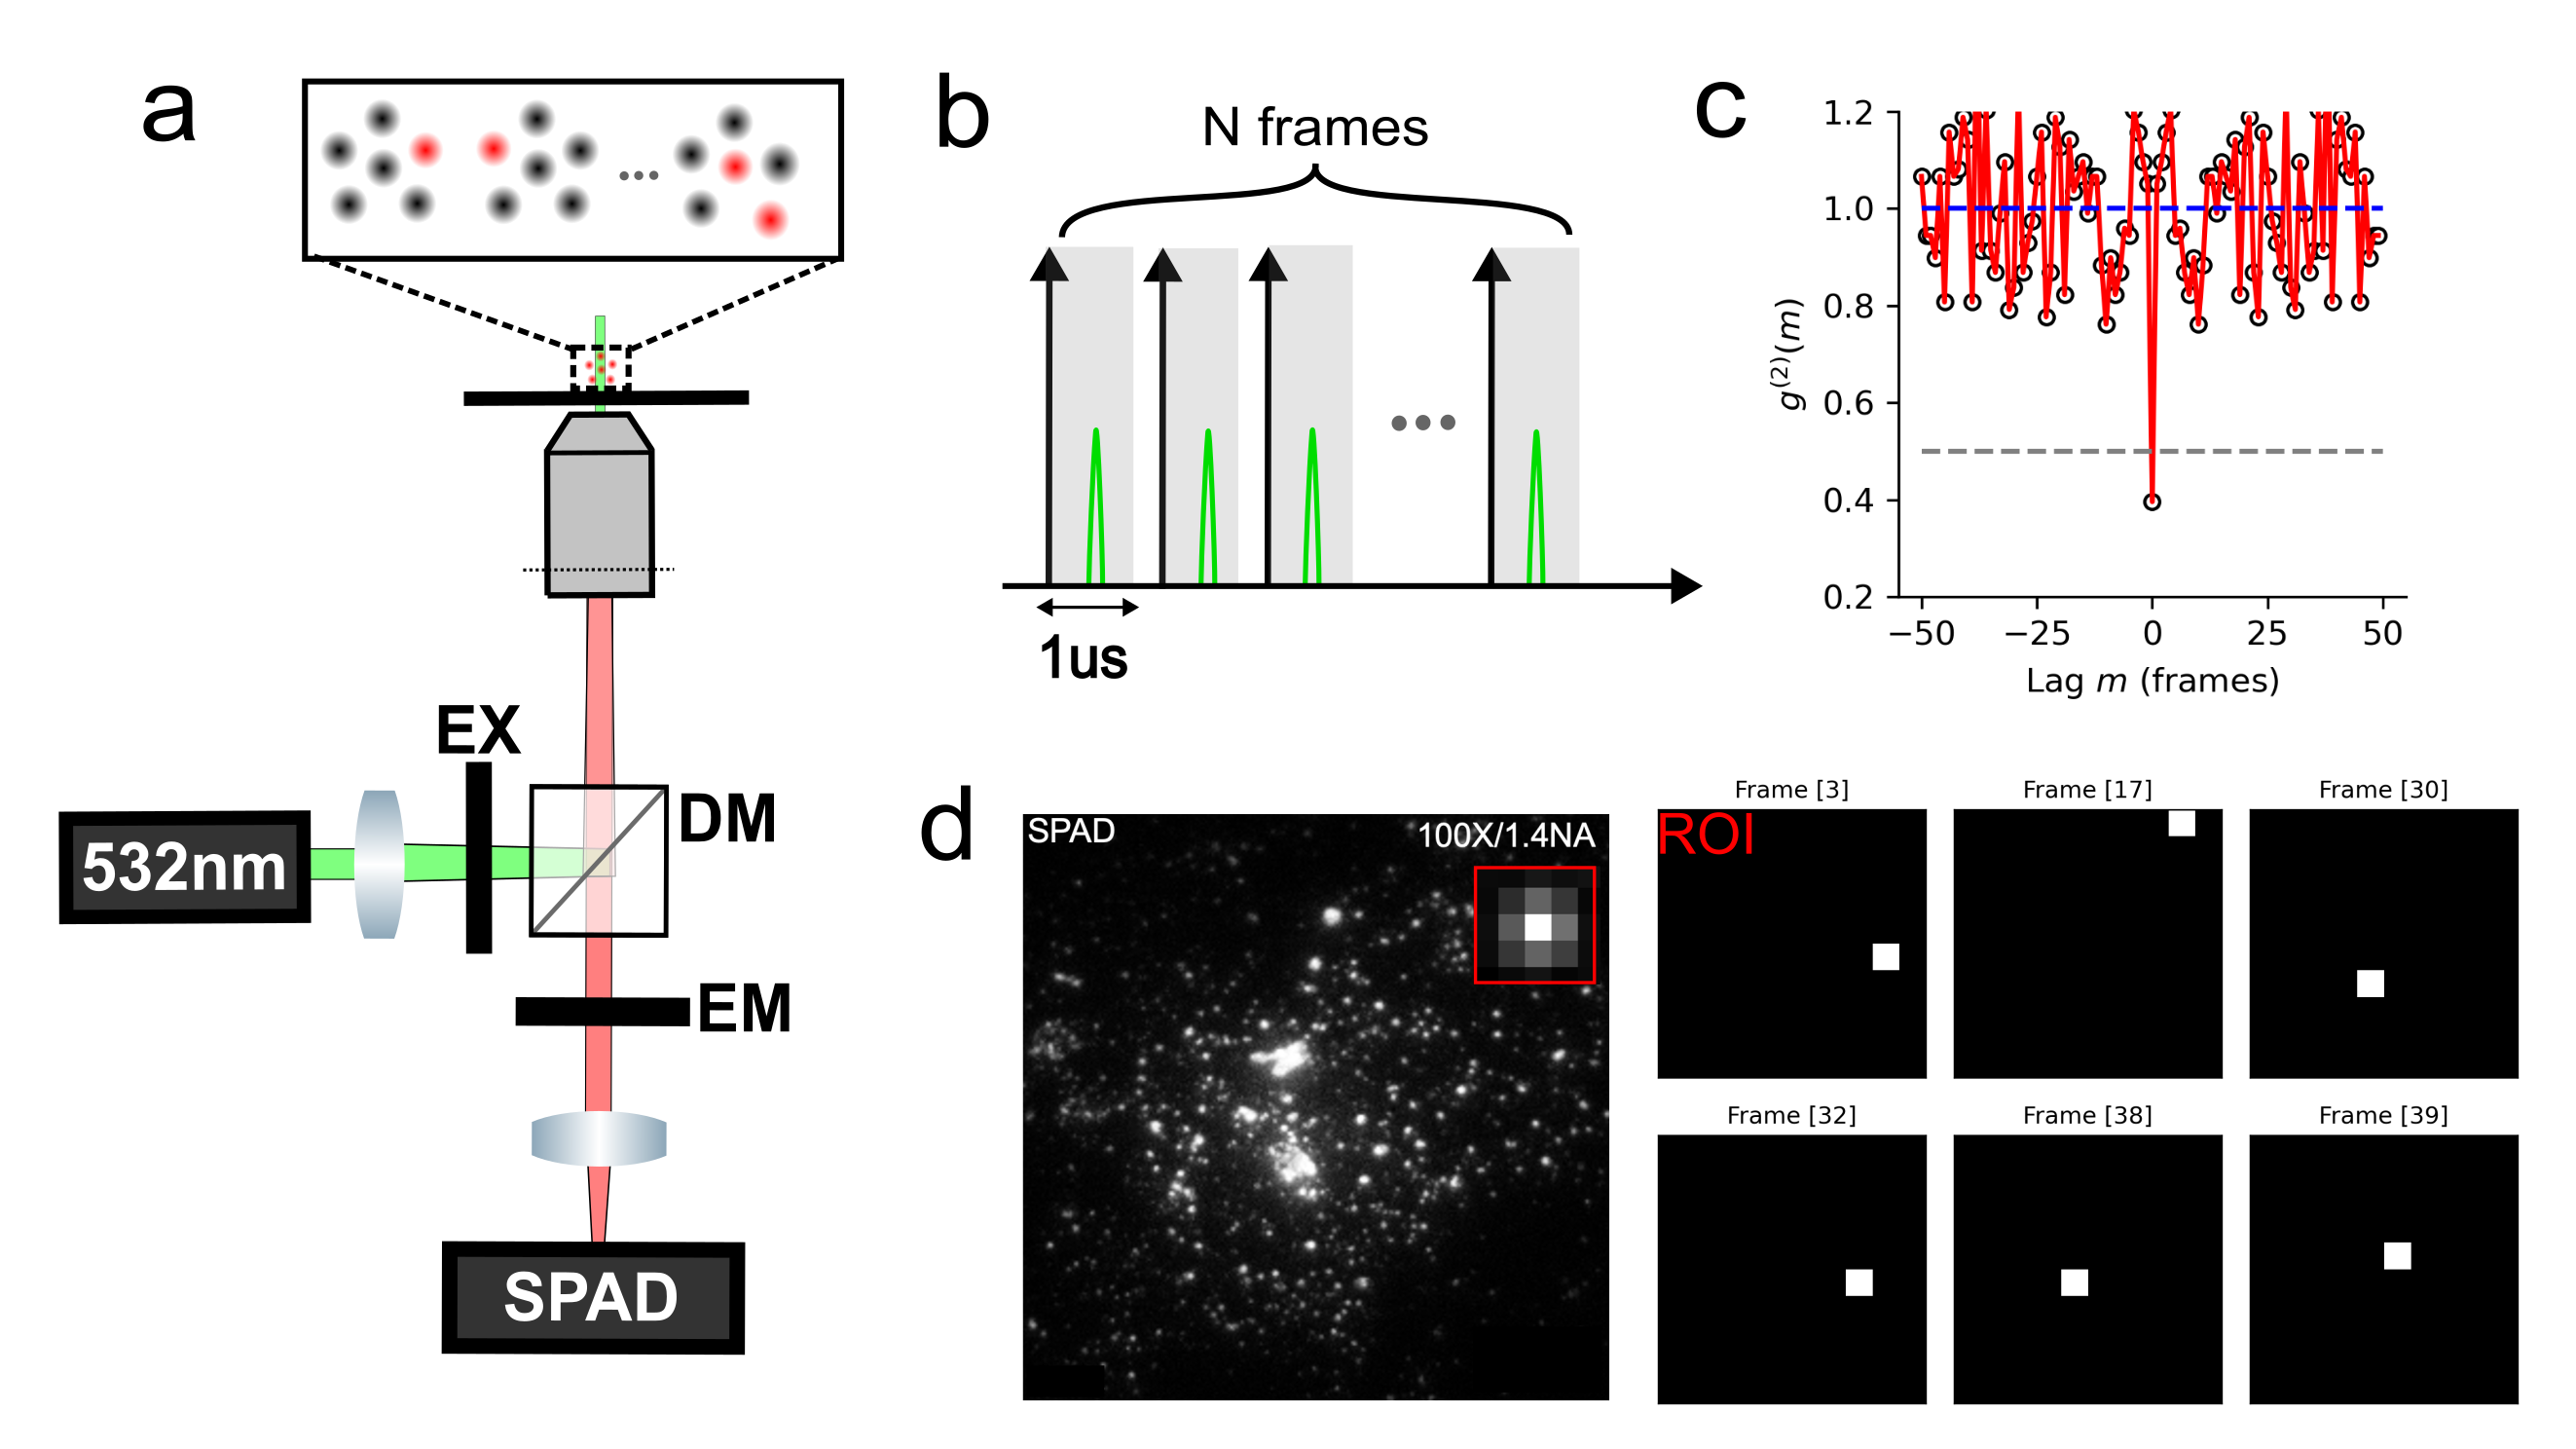
\includegraphics[width=16cm]{/Users/cwseitz/git/cwseitz.github.io/docs/phd/spad/spad/media/Figure-0.png}
\caption{\textbf{Single photon counting with a SPAD array} (a) Simplified diagram of the widefield photon counting setup (b) Single photon imaging scheme using 1us exposures containing a picosecond laser pulse (c) Sum of photon counts over a 5x5 region of interest (ROI), taken with $N_{\mathrm{frames}}=5\times 10^{5}$}
\label{fig:fig5}
\end{figure*}    

Consider a simplified description of widefield photon counting for a a single photon source in the object plane labeled by a continuous-valued coordinate $\theta=(\theta_u,\theta_v)$. The spatial profile $O$ of the field in image space is again presumed to have a Gaussian shape \parencite{Zhang2007,Richards1959,Gibson1989}. 

\begin{equation}
I(t)=\frac{W(t)}{2\pi\sigma^2}e^{-\frac{\left(u-\theta_u\right)^2+\left(v-\theta_v\right)^2}{2\sigma^2}}  
\end{equation}

In general, fluorescent emission is a doubly stochastic process \parencite{Chen1999}, due to temporal fluctuations in the intensity $W(t)$ as well as the quantum nature of light. We therefore define the molecular brightness $\zeta(t)\propto W(t)$ as the probability a photon is detected from a fluorescent emitter at a time $t$ . All factors that affect the photon count rate, such as laser power, absorption cross section, fluorescence quantum yield, detector efficiency, etc., are absorbed into $\zeta(t)$. Under stationary conditions in which $W(t)$ and $\zeta(t)$ are constants, we write $\zeta(t)=\zeta$. In this case, for an isolated single photon source, the PCH will follow a Bernoulli distribution: 

%A similar theoretical exposition to follows to Section 1.2; however, slight modifications are made to the notation to relate it to the quantum theory. Since our SPAD detectors at the image plane must also be discrete, the intensity at a detector element $k$ centered in image space at $s_k=(u_k,v_k)$ is given by integrating over pixels of width $\delta=1$. Using the definitions of $\Gamma_u,\Gamma_v$ from Section 1.2, we define

%\begin{equation}
%\zeta_{k}\vcentcolon = \langle n_{k} \rangle = \Gamma_{u}(u_k,\theta_u)\Gamma_{v}(v_k,\theta_v)\zeta
%\end{equation}

%where $\langle n_{k} \rangle$ is the expected number of photons detected at pixel $k$. We now consider the case of pulsed excitation where the interval between pulses is much longer than the fluorescence lifetime. Upon excitation of an isolated fluorescent emitter, a photon is detected at a particular detector element $k$ with probability $\zeta_{k}$. Similarly, the probability of detection in a region of interest collecting all photons is $\zeta$. Here, we are primarily concerned with the latter quantity, and its application in counting fluorescent emitters.

\begin{equation}
\mathcal{L}_{\mathrm{signal}}^{(1)}(n_{\mathrm{signal}}\lvert\zeta)\ =\ \mathrm{Bernoulli}(\zeta)
\end{equation}

If $N$ fluorescent emitters are present in the ROI, the PCH will be the $N$-th convolution of the single emitter PCH with itself \parencite{Chen1999}

\begin{equation}
\mathcal{L}_{\mathrm{signal}}(n_{\mathrm{signal}})=\mathcal{L}_{\mathrm{signal}}^{(1)}(\zeta_1)\otimes\mathcal{L}_{\mathrm{signal}}^{(2)}(\zeta_2)\otimes\ \cdots\otimes\mathcal{L}_{\mathrm{signal}}^{(N)}(\zeta_N)
\end{equation}

Therefore, for $N$ identical fluorophores emitting photons which can be detected within a ROI of the array, the number of signal photons measured $n_{\mathrm{signal}}$ following a single excitation pulse will have Binomial statistics $n_{\mathrm{signal}}\sim \mathrm{Binom}\left(N,\zeta\right)$. Photon pile-up at a single detector element can be safely neglected in this model due to its relatively low likelihood. Coherent background signal will follow Poissonian statistics $n_{\mathrm{bg}}\sim\mathrm{Poisson}\left(\lambda\right)$ for an expected number $\lambda$ of background counts in the ROI per frame. The total number of counts $n=n_{\mathrm{signal}}+n_{\mathrm{bg}}$ detected in the region of interest following a single pulse is then distributed by the PCH:

\begin{equation}
\mathcal{L}\left(n\mid N,\zeta,\lambda\right)=\mathcal{L}_{\mathrm{signal}}(n_{\mathrm{signal}}\lvert N,\zeta)\otimes\mathcal{L}_{\mathrm{bg}}(n_{\mathrm{bg}}\lvert \lambda)=\sum_{i=0}^{\infty}\binom{N}{i}\zeta^i\left(1-\zeta\right)^{N-i}\frac{\lambda^{n-i}}{\left(n-i\right)!}e^{-\lambda} 
\end{equation}

The expression above represents a convolution of Poisson and Binomial probability mass functions. This result is the primary means of inference of the number of active emitters $N$ in a ROI as well as theoretical analysis of the second-order coherence. 


%\begin{figure}[t]
%\centering
%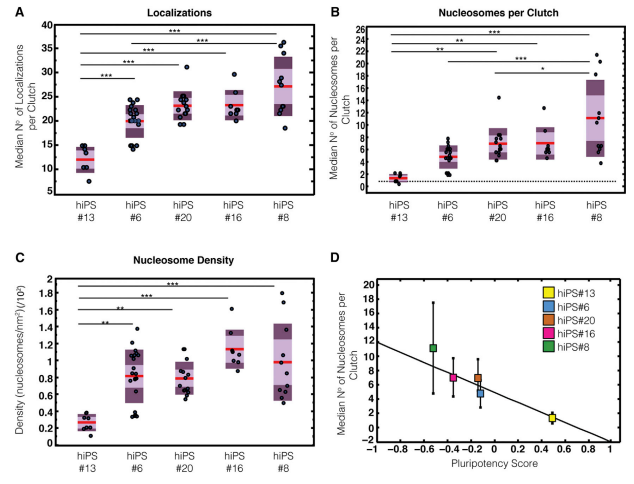
\includegraphics[width=12cm]{/Users/cwseitz/git/cwseitz.github.io/docs/phd/spad/spad/media/Figure-4.png}
%\caption{\textbf{Posteriors on the number of fluorescent emitters $N$ and localization for $N^{*}=1$} (left) and $N^{*}=2$ (right) quantum dots. Scalebars 360nm}
%\label{fig:fig7}
%\end{figure}


%By temporarily ignoring the spatial profile described by (2.3), we derive a likelihood on the number of fluorophores in a small ROI with a lateral dimension $d = 5$ pixels. For $N$ fluorophores emitting photons which can be detected within a ROI of the SPAD array, the number of signal photons measured $n_{\mathrm{signal}}$ following a single excitation pulse will have Binomial statistics $n_{\mathrm{signal}} \sim \mathrm{Binom}(N,\zeta)$. Photon pile-up at a single detector element can be safely neglected in this model due to its relatively low likelihood. We then model the background signal within the ROI as a coherent state, which we have shown follows Poissonian statistics $n_{\mathrm{background}} \sim \mathrm{Poisson}(\lambda)$ for an expected number $\lambda$ of background counts in the ROI, per frame. The total number of counts $n=n_{\mathrm{signal}}+n_{\mathrm{background}}$ detected in the ROI following a single pulse is then distributed by the likelihood

%\begin{equation}
%p(n \mid N,\zeta,\lambda) = \sum_{i=0}^{\infty} \binom{N}{i} \zeta^i (1-\zeta)^{N-i} \frac{\lambda^{n-i}}{(n-i)!} e^{-\lambda}
%\end{equation}

%The expression above represents a convolution of Poisson and Binomial probability mass functions. This result is the primary means of inference of the number of active emitters $N$ in a ROI.

%In order to begin to perform localization in non-sparse ROIs, we write a posterior distribution on the Binomial parameters used in the likelihood, using Bayes rule. Presuming $\lambda$ can be reliably estimated, we have

\subsubsection{Empirical estimation of second-order coherence}

To measure fluorescence antibunching in experiments, the second order coherence function $g^{(2)}(m)$ is used \parencite{Israel2017}. An empirical estimate of $g^{(2)}(m)$ is made, based on the number of coincidences $G^{(2)}(m)$ at a lag time $m$

\begin{equation}
g^{(2)}(m)=\frac{G^{(2)}(m)}{\langle G^{(2)}(m)\rangle }
\end{equation}


The function $G^{(2)}(m)$ counts the number of coincidences at a lag time $m$ and is normalized by its expectation $\langle G^{(2)}(m)\rangle$. It is well known that, for coherent (Poissonian) light, the second order coherence function $g^{(2)}(m)$ is approximately unity for all lags $m$. This is not necessarily the case, however, for binomial states \parencite{Stoler1985} of the quantized radiation field. To investigate the properties of the $g^{(2)}(0)$ dip for binomial photon statistics, we compared the expected number of coincidences at zero-lag $G^{(2)}(0)$ as well as the $g^{(2)}(0)$ value for purely binomial or Poissonian photon statistics, with the same mean. As expected, we found that binomial statistics gave a dip below $g^{(2)}(0) =0.5$ for small fluorophore numbers while Poissonian statistics gave a value of $g^{(2)}(0) =0.5$ (Figure \ref{fig:binomvpoiss}a). This result was also seen for pure binomial statistics (zero background signal) over a range of $\zeta$ values (Figure \ref{fig:binomvpoiss}b). For nonzero background signal, we find that the signal to background ratio becomes relevant, with decreasing $\zeta$ values raising the expected dip to $g^{(2)}(0) =0.5$ (Figure \ref{fig:binomvpoiss}c).


\subsubsection{Bayesian inference of the number of active emitters}

When the number of fluorescent emitters $N$ is unknown, the PCH (likelihood function) can be used in a Bayesian inference scheme to construct a posterior distribution on the binomial parameters:

\begin{equation}
p(N,\zeta\lvert n) \propto p(n\lvert N,\zeta)p(\zeta)
\end{equation}

We use a Gaussian prior on $\zeta$, i.e. $p(\zeta) = \mathcal{N}(\mu_{\zeta},\sigma_{\zeta}^2)$. Prior uncertainty in the value of $\zeta$ stems from fluorophores with potentially complex photophysical properties. This posterior can be integrated over $\zeta$ to produce a posterior distribution on the fluorophore number $N$. That is, $p(N=N'\lvert n) \propto \int_{0}^{1} \mathcal{L}(n\lvert N',\zeta)p(\zeta) d\zeta$ for $\mathcal{L}(n\lvert N',\zeta)=\prod_{j=1}^{N\mathrm{frames}} p(n_{j}\lvert N',\zeta)$. The likelihood is made tractable by a log-sum-exponential trick: $\mathcal{L}(n\lvert N',\zeta) = e^{\left(\sum_{j}\ell (n_{j}\lvert N',\zeta) + C\right)}$, where $C$ is an arbitrary constant determined empirically. This same constant $C$ is used for all $N'$. Monte Carlo integration is then employed to integrate out $\zeta$. This involves sampling many $\zeta$ values from the Gaussian prior and, for each sampled $\zeta$, the Poisson-Binomial likelihood $\mathcal{L}(n\lvert N',\zeta)$ is computed. These likelihood values are then weighted by the prior probabilities $p(\zeta_i)$. The final result is obtained by averaging these weighted likelihoods over all sampled $\zeta$, which approximates the integral:

\begin{equation}
p(N=N'\lvert n) = \int_{0}^{1} \mathcal{L}(n\lvert N',\zeta) p(\zeta) \, d\zeta \approx \frac{1}{S} \sum_{i=1}^S \mathcal{L}(n\lvert N',\zeta_i) p(\zeta_i)
\end{equation}

where $S$ is the number of samples from the prior. This method provides a powerful way to handle the integration of complex or high-dimensional functions, especially when analytical solutions are intractable. The final posterior can then be estimated by minibatching the data and averaging the posterior $p(N\lvert n)$ over minibatches. An estimate of the fluorophore number $N$ within each ROI is found by the maximum aposteriori (MAP) estimate $N^{*}$ given by this distribution.

%For localization, we notice that the Poisson-Binomial likeliood is well approximated by a Poisson distribution for $\zeta << 1$, making the localization procedure similar to conventional maximum likelihood methods discussed in Chapter 1. Therefore, we have the following log-likelihood on the image $\bold{x}$:


%\begin{equation}
%\ell(\bold{x}\lvert \theta) = -\log \prod_{k} \frac{e^{-\left(\mu_{k}\right)}\left(\mu_{k}\right)^{n_k}}{n_k!}\\
%= \sum_{k}  \log n_k! + \mu_{k} - n_k\log\left(\mu_{k}\right)
%\end{equation}

%\begin{figure*}[t]
%\centering
%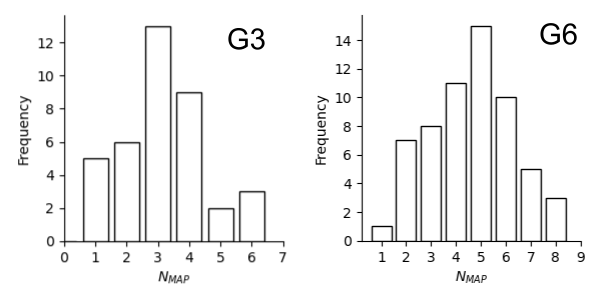
\includegraphics[width=12cm]{/Users/cwseitz/git/cwseitz.github.io/docs/phd/spad/spad/media/Figure-5.png}
%\caption{\textbf{Single and multi-emitter localization error on sums of photon counts}. (left) Localization uncertainty for simulated data for different values of $N$, plotted with respect to the Cramer-Rao lower bound, shown in dashed gray. (right) Multi-emitter localization by MCMC sampling for $N=3$, colors indicate a cluster of samples i.e., a single localization. All data was generated with a background rate $\langle n_{\mathrm{background}} \rangle = \lambda N_{\mathrm{frames}}/d^{2}$ per pixel. Scalebar 360nm}
%\label{fig:fig6}
%\end{figure*}   

%where, in the multi-emitter regime the expected photon count at a pixel is $\mu_{k} = \sum_{m=1}^{N^{*}} \mu_{k,m}$ and $\mu_{k,m}=\zeta N_{\mathrm{frames}}\Gamma_{x}(u_k,\theta_{u,m})\Gamma_{y}(v_k,\theta_{v,m}) + \lambda N_{\mathrm{frames}}/d^{2}$. In the multi-emitter regime, optimization of the likelihood can be more challenging, and sampling is a more suitable choice compared to gradient-based methods (see Results). 

\subsubsection{Simulations}

\begin{figure}
\centering
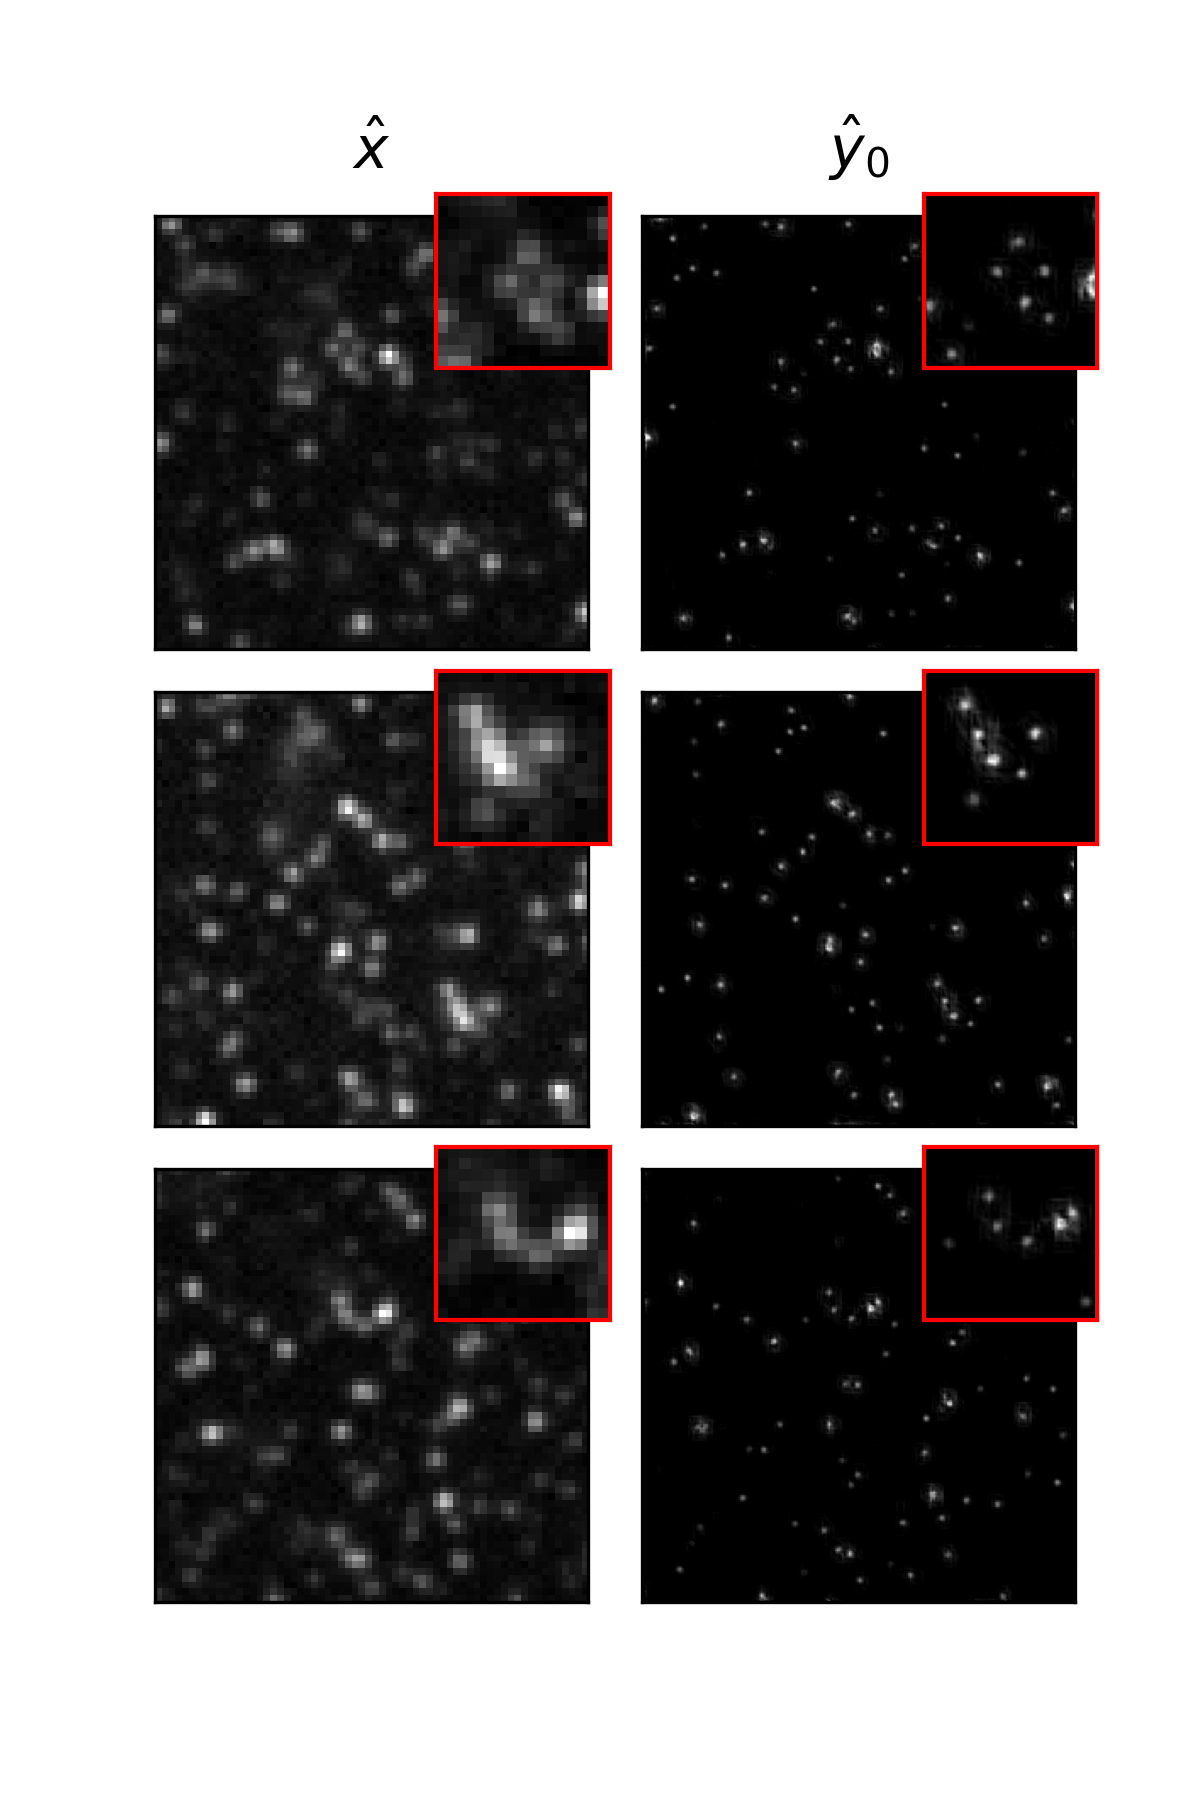
\includegraphics[width=16cm]{/Users/cwseitz/git/cwseitz.github.io/docs/phd/spad/spad/media/Figure-6.png}
\caption{\textbf{Photon counting histogram and analysis on zero-background simulations} (a) Simulated photon counts in 1us exposure for $N=1$ and $\zeta=0.01$ (b) Photon counting histogram for counts in (a) (c) Second-order coherence function for data in (a) (d) Posterior distribution for data in (a) (e) Simulated photon counts in 1us exposure for $N=1$ and $\zeta=0.01$ (f) Photon counting histogram for counts in (e) (g) Second-order coherence function for data in (e) (h) Posterior distribution for data in (e) (i) Simulated photon counts in 1us exposure for $N=1$ and $\zeta=0.01$ (j) Photon counting histogram for counts in (i) (k) Second-order coherence function for data in (i) (l) Posterior distribution for data in (i) Inference in (d,h,l) use $\mu_\zeta=0.01,\sigma_\zeta=0.001$}
\label{fig:pch}
\end{figure}  

To validate our model, we apply it on the simulated photon emissions from single and multiple quantum emitters. Simulated photon count time-series were generating by sampling from the Poisson-Binomial PCH described using variable values for $N$ and $\zeta=0.01$ (Figure \ref{fig:pch}a,e,i). As expected, we found that $g^{(2)}(0)<0.5$  while for increasing values of $N$, $g^{(2)}(0)$ approached $g^{(2)}(0)=0.5$ (Figure \ref{fig:pch}c,g,k). Analysis of the posterior distribution on $N$ successfully recovered the value of $N$ used to parameterize simulations (Figure \ref{fig:pch}d,h,l). 

\subsubsection{Distinguishing single quantum dots from assemblies}

A custom widefield fluorescence microscope was built for widefield photon counting by synchronization of laser pulses with 1-bit exposures of a SPAD array. This excitation scheme permits the computation of the second order coherence function  $g^{(2)}(m)$ and visualization of the spatial intensity distribution by summing photon counts over time. The acquisition scheme and analytical methods were then applied in two experimental contexts. First, we examined the posterior distribution and $g^{(2)}(m)$ function for putatively isolated quantum dots and then examined quantum dot aggregates. Quantum dots exhibit temporally heterogeneous photoluminescence (PL) due to nonradiative transitions of electrons in the conduction band giving rise to a phenomenon known as blinking \parencite{Stoler1985,Furuta2022}. Quantum dots showing clear two-state PL fluctuations exhibited $g^{(2)}(0)<0.5$ and a posterior distribution maximized at $N=1$ (Figure \ref{fig:qdagg}a-d). Aggregates of quantum dots with more complex PL fluctuations showed $g^{(2)}(0)=0.5$ and a posterior distributed around larger values of $N$ (Figure \ref{fig:qdagg}e-h) 

\begin{figure}
\centering
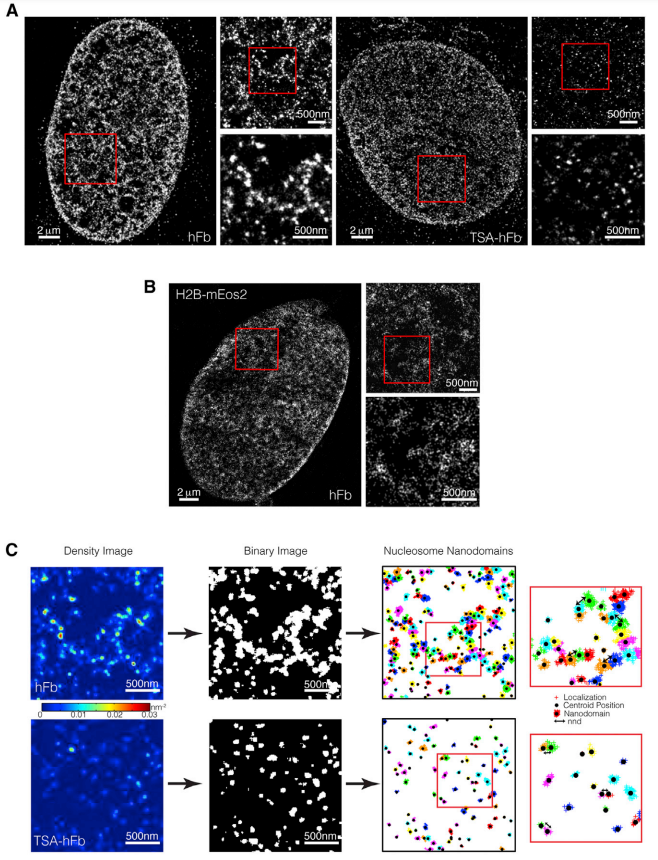
\includegraphics[width=16cm]{/Users/cwseitz/git/cwseitz.github.io/docs/phd/spad/spad/media/Figure-1.png}
\caption{\textbf{Distinguishing single and multiple quantum dots} (a) Photon counts in 1us exposure using 532nm pulsed excitation of a putatively isolated QD (b) Photon counts in 10ms exposure using 488nm continuous-wave excitation (c) Second-order coherence function for data in (a) (d) Posterior distribution for data in (a) (e) Photon counts in 1us exposure using 532nm pulsed excitation of a QD aggregate (f) Photon counts in 10ms exposure using 488nm continuous-wave excitation (g) Second-order coherence function for data in (e) (h) Posterior distribution for data in (e). Inference parameters can be found in Table 1.}
\label{fig:qdagg}
\end{figure}  

\clearpage
\begin{figure}
\centering
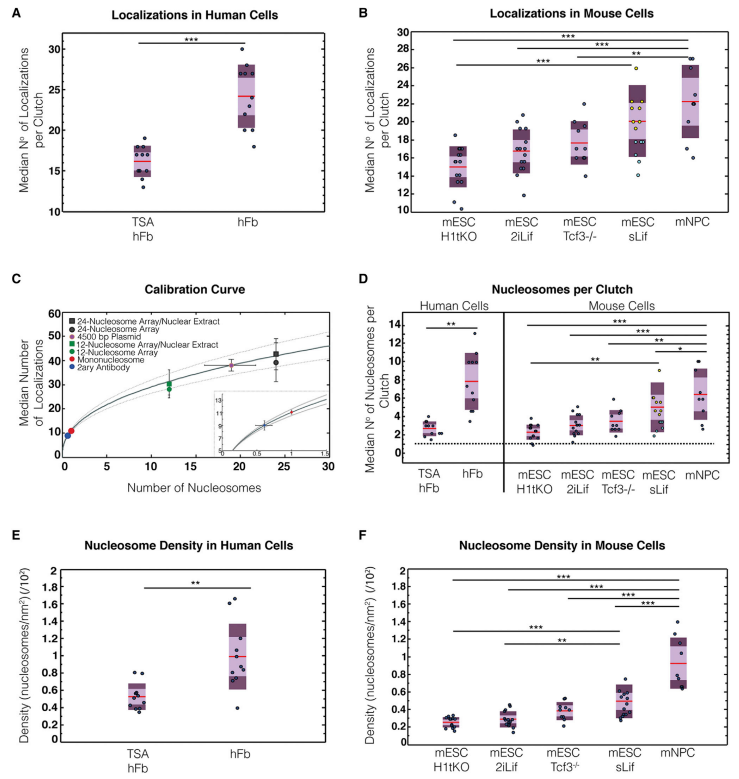
\includegraphics[width=16cm]{/Users/cwseitz/git/cwseitz.github.io/docs/phd/spad/spad/media/Figure-3.png}
\caption{\textbf{Counting ATTO532 dye bound to DNA origamis} (a) Example DNA origami with three ATTO532 binding sites (b) Photon counts in 1us exposure using 532nm pulsed excitation of G3 sample and sum of counts (inset) (c) Second order coherence for the spot in (b) (d) Posterior distribution for the spot in (b) (e) Example DNA origami with three ATTO532 binding sites (f) Photon counts in 1us exposure using 532nm pulsed excitation of G3 sample and sum of counts (inset) (g) Second order coherence for the spot in (f) (h) Posterior distribution for the spot in (f) (i) Example DNA origami with six ATTO532 binding sites (G6 sample) (j) Photon counts in 1us exposure using 532nm pulsed excitation of G6 sample and sum of counts (inset) (k) Second order coherence for the spot in (j) (l) Posterior distribution for the spot in (j).}
\label{fig:atto}
\end{figure}  

\clearpage
\begin{figure}
\centering
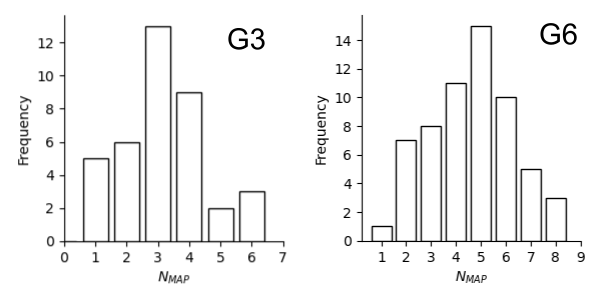
\includegraphics[width=12cm]{/Users/cwseitz/git/cwseitz.github.io/docs/phd/spad/spad/media/Figure-5.png}
\caption{\textbf{Distributions of the maximum aposteriori estimate of $N$} (left) Distribution of estimate of $N$ for DNA origamis with three ATTO532 binding sites (G3 sample) (right) Distribution of estimate of N for DNA origamis with six ATTO532 binding sites (G3 sample). Inference parameters can be found in Table 1.}
\label{fig:atto2}
\end{figure}  

\subsubsection{Counting fluorophores bound to DNA origamis}


In a second series of experiments, we examined the posterior distribution and $g^{(2)}(m)$ function for DNA origamis which can bind up to $N=3$ or $N=6$ ATTO532 fluorescent dye molecules, referred to as G3 and G6, respectively (Figure \ref{fig:atto}a,f,j) For origamis which can bind up to $N=3$ ATTO532 dyes, no clear $g^{(2)}(0)$ dip was observed, due to the low signal to background ratio at this signal level (Figure \ref{fig:atto}c,g). For origamis which can bind up to $N=6$ ATTO532 dyes, no clear $g^{(2)}(0)$ dip was observed, due to the large $N$ character of the $g^{(2)}(0)$ dip predicted by the theory (Figure \ref{fig:atto}k). We conclude that the $g^{(2)}(0)$ dip may lead to ambiguous interpretations at low signal levels. However, the posterior distribution can recover the known $N$ value from the photon count distribution for G3 (Figure \ref{fig:atto}d,h) and G6 (Figure \ref{fig:atto}l). Maximum aposteriori (MAP) estimates of the fluorophore number showed consistency with the known value of $N$ for G3 and G6 (Figure \ref{fig:atto2}). 

\clearpage
\begin{table}
\centering
\begin{tabular}{lccccc}
\multicolumn{6}{c}{\textbf{Table 1 - Posterior Parameters}} \\ \hline
\multicolumn{1}{c}{\textbf{Sample}}  & $\mu_{\zeta}$ & $\sigma_{\zeta}$ & $\lambda$ & Samples & Batches \\
Qdot655 & 0.01 & 0.005 & 0.008 & 100 & 50 \\
ATTO532 & 0.002 & 0.001 & 0.006 & 100 & 50 \\
\end{tabular}
\end{table}

\subsection{Materials and Methods}

\subsubsection{Quantum dots and DNA origamis preparation}

Fluorescent samples used here were either Quantum dots (Qdot655, ThermoFisher) coated on a glass coverslip, or ATTO532 tagged DNA origamis (GATTAquant). Fluorophores in a region with quasi-uniform laser power were selected for analysis to simplify the prior distribution on the molecular brightness. DNA origami samples contained origamis with either three or six ATTO532 binding sites for testing the Bayesian inference scheme and second-order coherence analysis. 

\subsubsection{Single molecule imaging with the SPAD array}

A 512x512 Fluorescent SPAD512 array (Pi Imaging Technologies) was connected to a custom single molecule imaging system (ASI). A picosecond 532nm pulsed laser (Picoquant) was triggered at 500 KHz as the excitation source. Laser power was set at 300uW at the back focal plane of the microscope objective for all experiments. Emission light was collected using an oil-immersion 100X/1.4NA objective (Nikon). The emission signal was filtered to exclude the laser line (Semrock) and projected onto the SPAD512 sensor using a tube lens. The acquisition of the SPAD assay is synchronized with the pulsed laser frequency. Each acquisition consists of a series of 1-bit frames, using a 1us exposure per frame. For quantum dot imaging, 30ms total exposure was used (30k frames). For DNA origami imaging, 100ms total exposure was used (100k frames). To obtain time-course data of photon counts, we (i) summed binary images over the entire acquisition (ii) estimated spot centroids using the Laplacian of Gaussian (LoG) detection algorithm, and (iii) extracted total counts in a 5x5 pixel region of interest around each detected spot. 


%Quantum dots coated on a glass coverslip were excited using a picosecond $532\mathrm{nm}$ pulsed laser triggered at $500\mathrm{kHz}$. Emission light was collected using an oil-immersion 100$\times$ objective with numerical aperture (NA) 1.4 (Nikon). The emission signal was then filtered to exclude the laser line (Semrock) and projected onto the SPAD512 sensor (Pi Imaging Technologies) using a tube lens. A simplified diagram of the complete system is depicted in (Figure \ref{fig:fig5} a). Each acquisition consists of $N=5\times 10^{5}$ frames, synchronized with each laser pulse, using a $1\mathrm{us}$ exposure per frame (Figure \ref{fig:fig5} b,d). Example posteriors and multi-emitter fitting on experimental quantum dot data are found in (Figure \ref{fig:fig7}). To measure fluorescence antibunching in the sample, we investigated properties of the zero-lag second order coherence function $g^{(2)}(0)$. The following empirical estimate of $g^{(2)}(0)$ is used \parencite{Israel2017}

%\begin{equation}
%g^{(2)}(0) = \frac{G^{(2)}(0)-B}{\langle G^{(2)}(m\neq 0)\rangle -B}
%\end{equation}

%\begin{figure}[t]
%\centering
%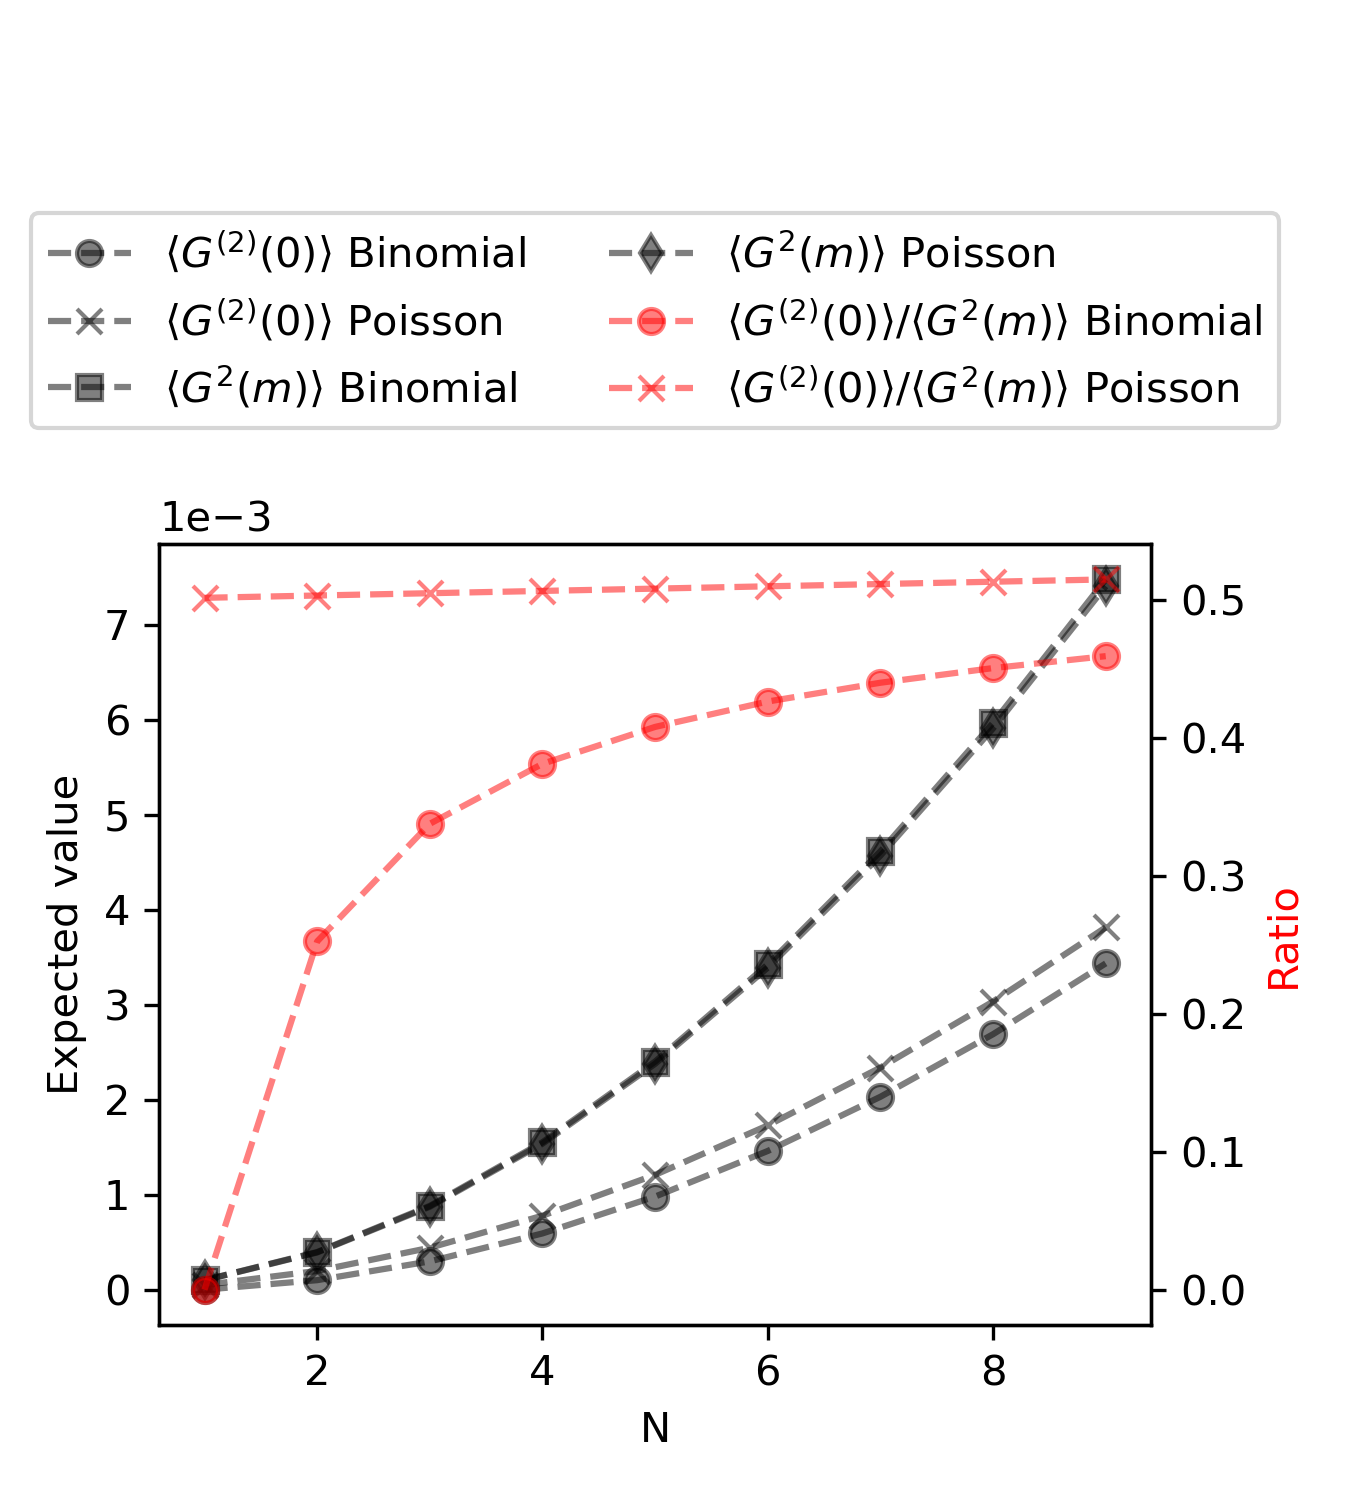
\includegraphics[width=12cm]{/Users/cwseitz/git/cwseitz.github.io/docs/phd/spad/spad/media/binomvpoiss.png}
%\caption{\textbf{Discrepancy of $g^{(2)}(0)$ for pure Binomial or Poissonianian data}. Binomial and Poisson distributions are similar for small $\zeta$ and large $N$. However, for small $N$, the Binomial $g^{(2)}(0)$ deviates from the Poisson $g^{(2)}(0)$ due to a small reduction in $\langle G^{(2})(0)\rangle$ (probability of zero-lag coincidence) in the Binomial case.}
%\label{fig:binomvpoiss}
%\end{figure}   

%\begin{figure}[t]
%\centering
%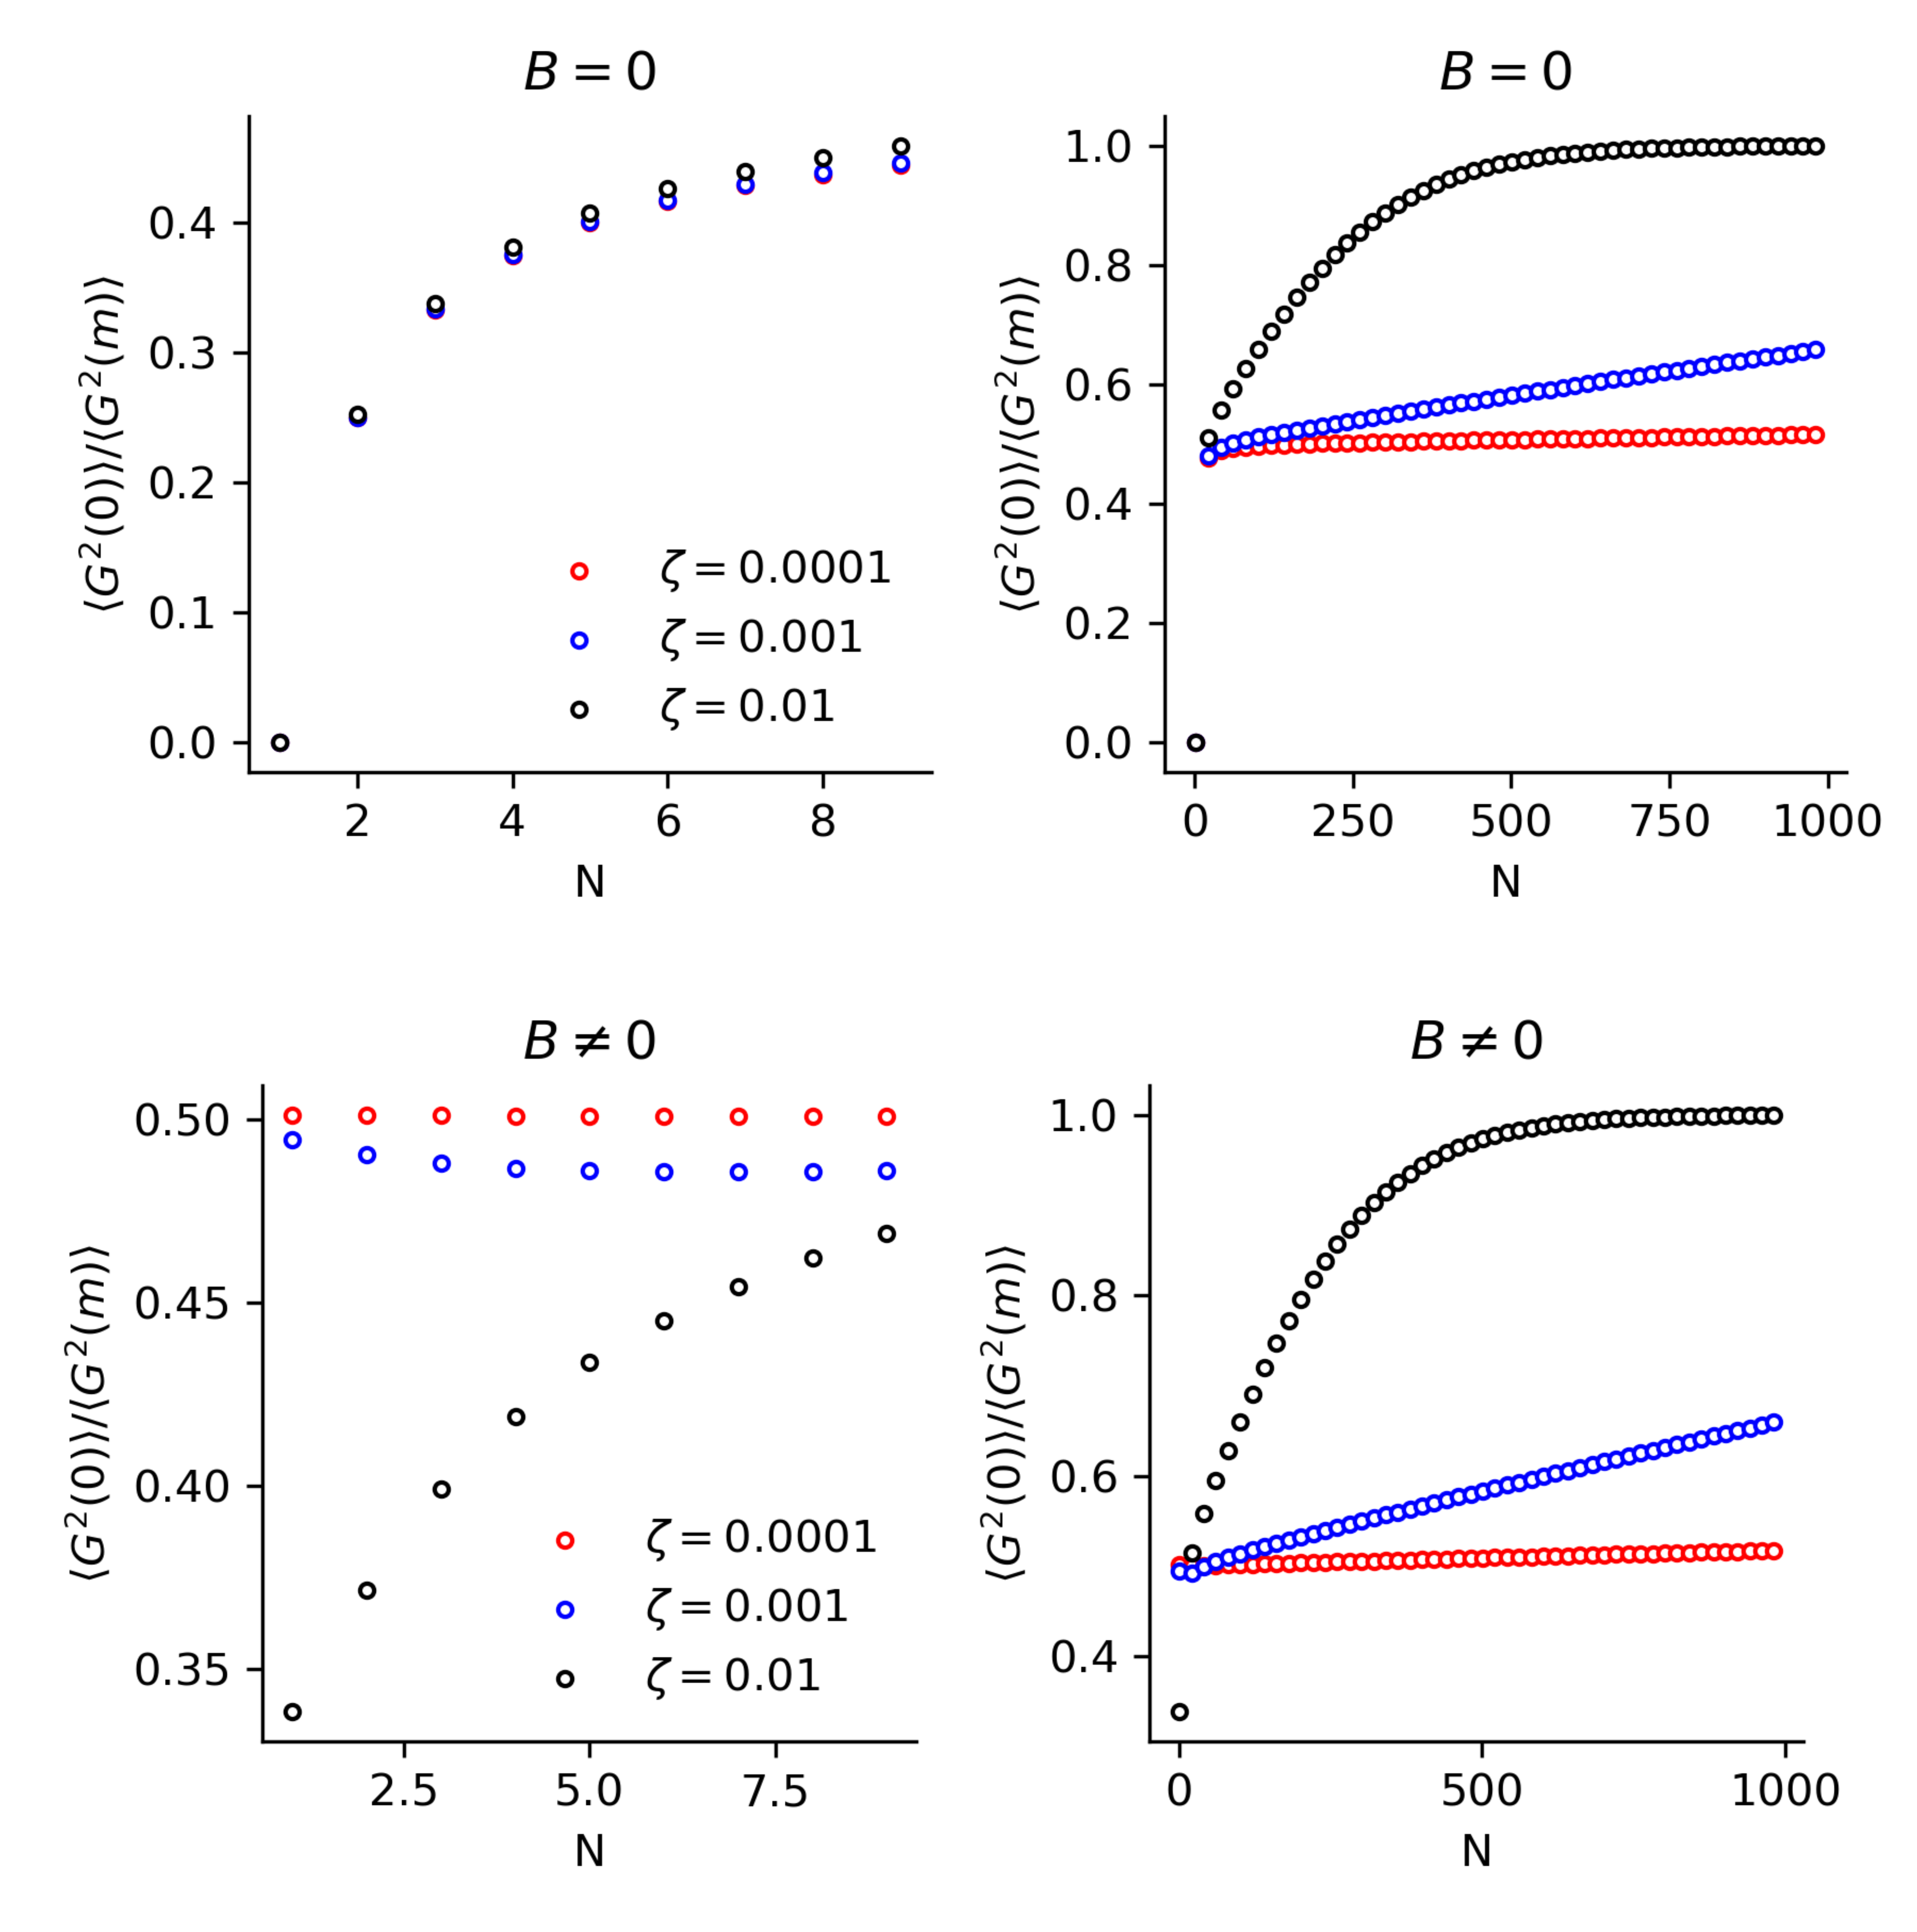
\includegraphics[width=12cm]{/Users/cwseitz/git/cwseitz.github.io/docs/phd/spad/spad/media/g20g2m_full.png}
%\caption{\textbf{Theoretical scaling of $g^{(2)}(0)$ under zero and non-zero background conditions without correction}. (left) Scaling of $g^{(2)}(0)$ for small $N$. (right) Scaling of $g^{(2)}(0)$ for large $N$. For non-zero background conditions, $\lambda = 0.0075$. For small $\zeta$, $g^{(2)}(0)\approx 0.5$, which is the value for Poisson statistics}
%\label{fig:fig8}
%\end{figure}   

%where $B = N_{\mathrm{frames}}\lambda\zeta$ is the expected number of background-signal coincidences in the region of interest. The quantity $G^{(2)}(m)$ represents the number of signal-signal coincidences in the region of interest at a lag time $m$. The quantity $\langle G^{(2)}(m\neq 0)\rangle$ is the average number of coincidences in pairs of frames at nonzero lag $m \in [1,100]$, in units of frames. Averaging $G^{(2)}(0)$ over many realizations (sequences of $N_{\mathrm{frames}}$), gives the expected value $\langle G^{(2)}(0)\rangle $

%\begin{equation}
%\langle G^{(2)}(0)\rangle = N_{\mathrm{frames}}(1 - (1-\zeta)^N - N\zeta (1-\zeta)^{N-1})
%\end{equation}

%Since $G^{(2)}(m)$ is already averaged over $m$, $\langle G^{(2)}(m) $ is effectively a constant over realizations, and must be

%\begin{equation}
%\langle G^{(2)}(m)\rangle =  N_{\mathrm{frames}} \left(1 - \left((1-\zeta)^N\right)\right)^2
%\end{equation}

%Ignoring the effect of background signal $\langle g^{(2)}(0)\rangle =\langle G^{(2)}(0)\rangle/\langle G^{(2)}(m)\rangle$, which rapidly approaches $1/2$ as a function of $N$, and then saturates and slowly while approaching a maximum value of 1 (Figure \ref{fig:fig8}). This is consistent with the idea that for very large number of active fluorescent emitters, the statistics should become Poisson. Lastly, $G^{(2)}(0),G^{(2)}(m),B$ all will have Binomial statistics, which can approximated as Poisson for $\zeta << 1$. Error estimates are then $\delta G^2(0) = \sqrt{G^2(0)}, \delta E(G^2(m)) = \sqrt{\frac{\mathbb{E}(G^2(m))}{M}}, \delta B = \sqrt{B}$. This gives the following error in the value of $g^{(2)}(0)$:

\subsubsection{Computation of the second order coherence}

In practice, we compute the second order coherence at zero lag using

\begin{equation*}
G^{(2)}(0) =\ \sum_{t}{\mathbb{I}(n_t>1)}
\end{equation*}

where $\mathbb{I}$ is an indicator function. The value of this function at nonzero lag $m$ is given by

\begin{equation*}
G^{(2)}(m) =\ \sum_{t}{\mathbb{I}(n_t n_{t+m}\geq1)}
\end{equation*}

The second order coherence $g^{(2)}(m)$ is then computed over a range $-m_{min}\le m\le m_{max}$. Theoretical estimates of $g^{(2)}(0)$ can be obtained by determining the generating model of $G^{(2)}(m)$. We find that for a sequence of $M$ frames,

\begin{equation*}
G^{(2)}(0)\sim \mathrm{Binomial}(M,p)\ \ \ \ p=\sum_{n\geq2}{\mathcal{L}(n\lvert N,\zeta)}
\end{equation*}

\begin{equation*}
G^{(2)}(m)\sim \mathrm{Binomial}\left(M,q\right)\ \ \ \ \ q=\left(\sum_{n\geq1}{\mathcal{L}(n\lvert N,\zeta)}\right)^2
\end{equation*}

Fluorescence antibunching is conventionally characterized by a dip in the $g^{(2)}(m)$ function for $m=0$, indicating a reduced coincidence probability. Error in the estimate of $g^{(2)}(0)$ are found by the expression


\begin{equation}
\sigma = \text{RMSE}[g^{(2)}(0)] = \sqrt{
    \left[
    \frac{\partial g^{(2)}(0)}{\partial \langle G^{(2)}(m) \rangle} \delta \langle G^{(2)}(m) \rangle
    \right]^2 +
    \left[
    \frac{\partial g^{(2)}(0)}{\partial G^{(2)}(0)} \delta G^{(2)}(0)
    \right]^2
}
\end{equation}

One can then integrate a Gaussian with this $\sigma$ below a threshold e.g, $g^{(2)}(0)=0.5$ to obtain the confidence interval. Lastly, $G^{(2)}(0),G^{(2)}(m)$ will have Binomial statistics, which we approximate as Poisson for simplicity. Error estimates are then $\delta G^2(0) = \sqrt{G^2(0)}, \delta \langle G^2(m)\rangle = \sqrt{\frac{\langle G^2(m)\rangle}{M}}$.This expression simplifies considerably in the case that $\delta \langle G^{(2)}(m)\rangle$ i.e., certainty in $G^{(2)}(m)$. 

\begin{equation}
\sigma_{g^{(2)}(0)}=\sqrt{\frac{p(1-p)}{M q^{2}}}
\end{equation}

The value of $\sigma_{g^{(2)}(0)}$ is therefore a function of $\zeta$ as well as the number of frames in the acquisition $M$. 


%For localization, we use Goodman and Weare's Markov Chain Monte Carlo (MCMC) algorithm \parencite{Goodman2010} to sample from the posterior on fluorophore locations. In all simulations we assume a uniform prior on coordinates over the ROI and $\zeta$ is known and identical over fluorophores. Fluorophore locations can then be estimated from the posterior samples by K-means clustering of the $(\theta_u,\theta_v)$ coordinates of the first particle and identification of cluster centers. To validate our estimator, we compare its RMSE to the single emitter CRLB. We find that for thousands of expected signal photon counts, localization uncertainty lies in an acceptable range for localization microscopy (Figure \ref{fig:fig6}).



%\begin{figure}
%\centering
%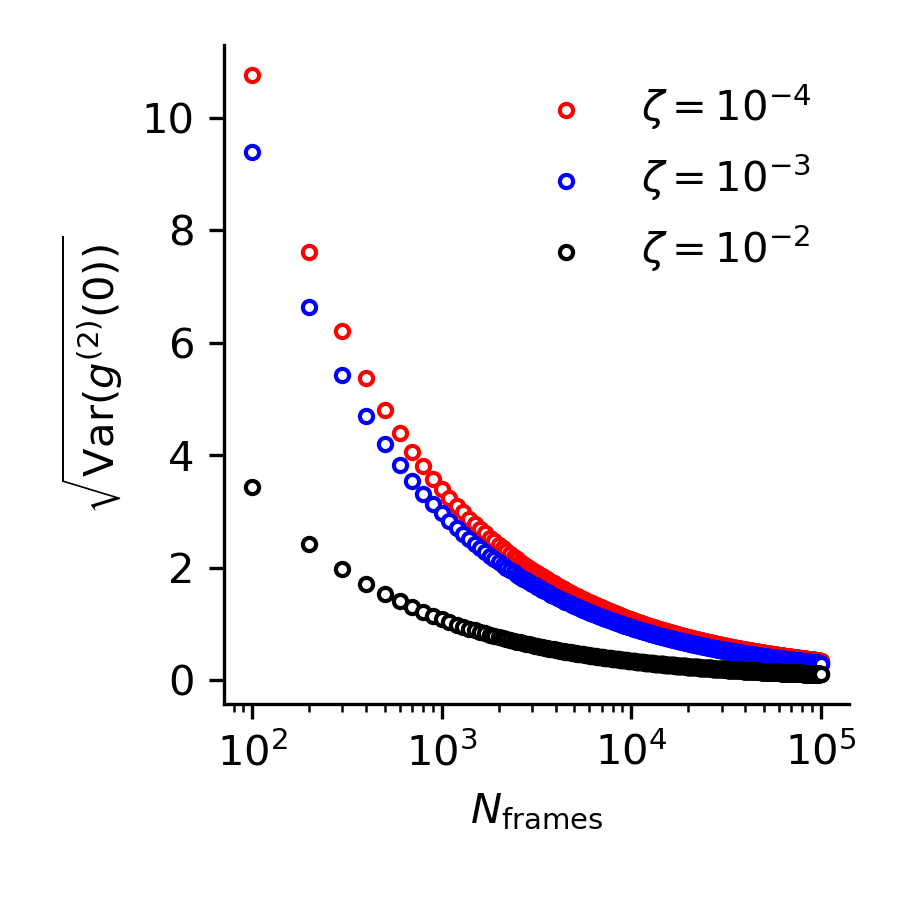
\includegraphics[width=8cm]{/Users/cwseitz/git/cwseitz.github.io/docs/phd/spad/spad/media/g20g2m_3.png}
%\caption{\textbf{Error in the second-order coherence dip}. Precision of the $g^{(2)}(0)$ estimate depends on the number of total frames (total photons) collected in the sequence. }
%\label{fig:atto}
%\end{figure}  



%\begin{figure*}[t]
%\centering
%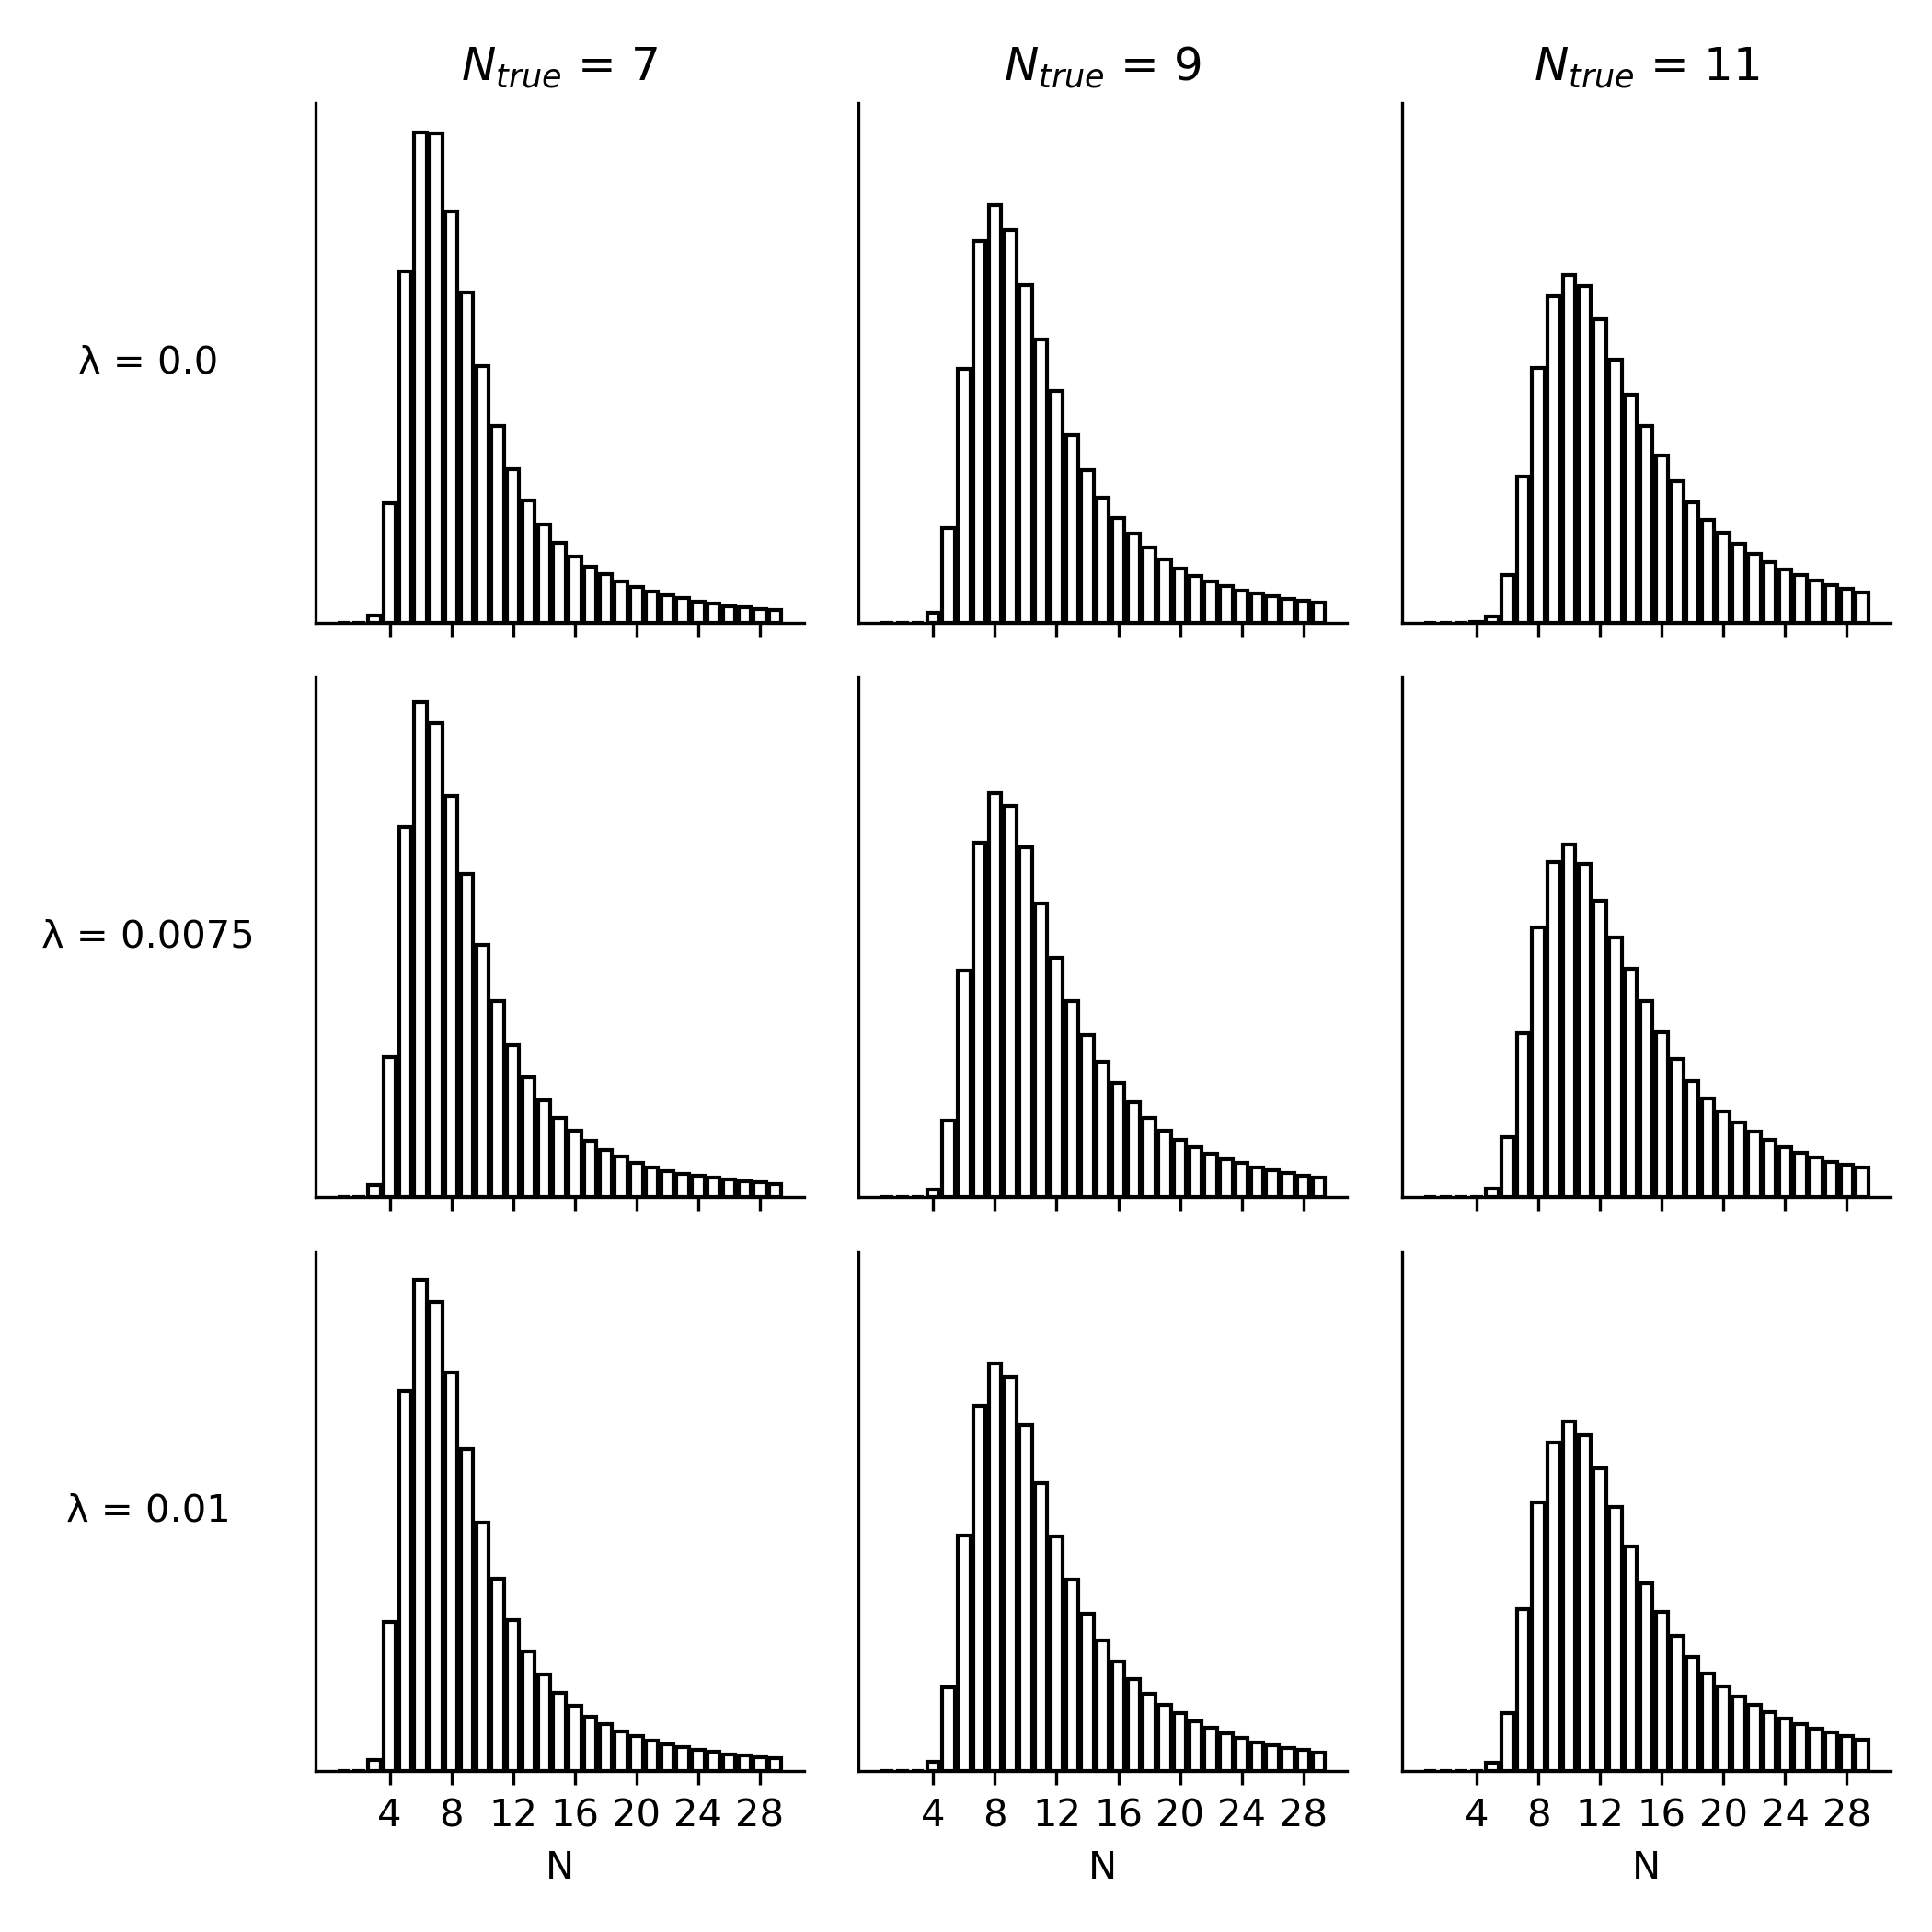
\includegraphics[width=14cm]{/Users/cwseitz/git/cwseitz.github.io/docs/phd/spad/spad/media/PoissonBinomialPost-2.png}
%\caption{\textbf{Posterior distributions of the fluorophore number}. Samples from the Poisson-Binomial convolution distribution using $\zeta=0.01$ for various values of $\lambda$ and $N=7,9,11$ were simulated. The variable $\zeta$ was integrated out by Monte Carlo integration, sampling 1000 $\zeta$ values from the posterior distribution (see main text for details)}
%\label{fig:fig10}
%\end{figure*}    

%\begin{figure*}[t]
%\centering
%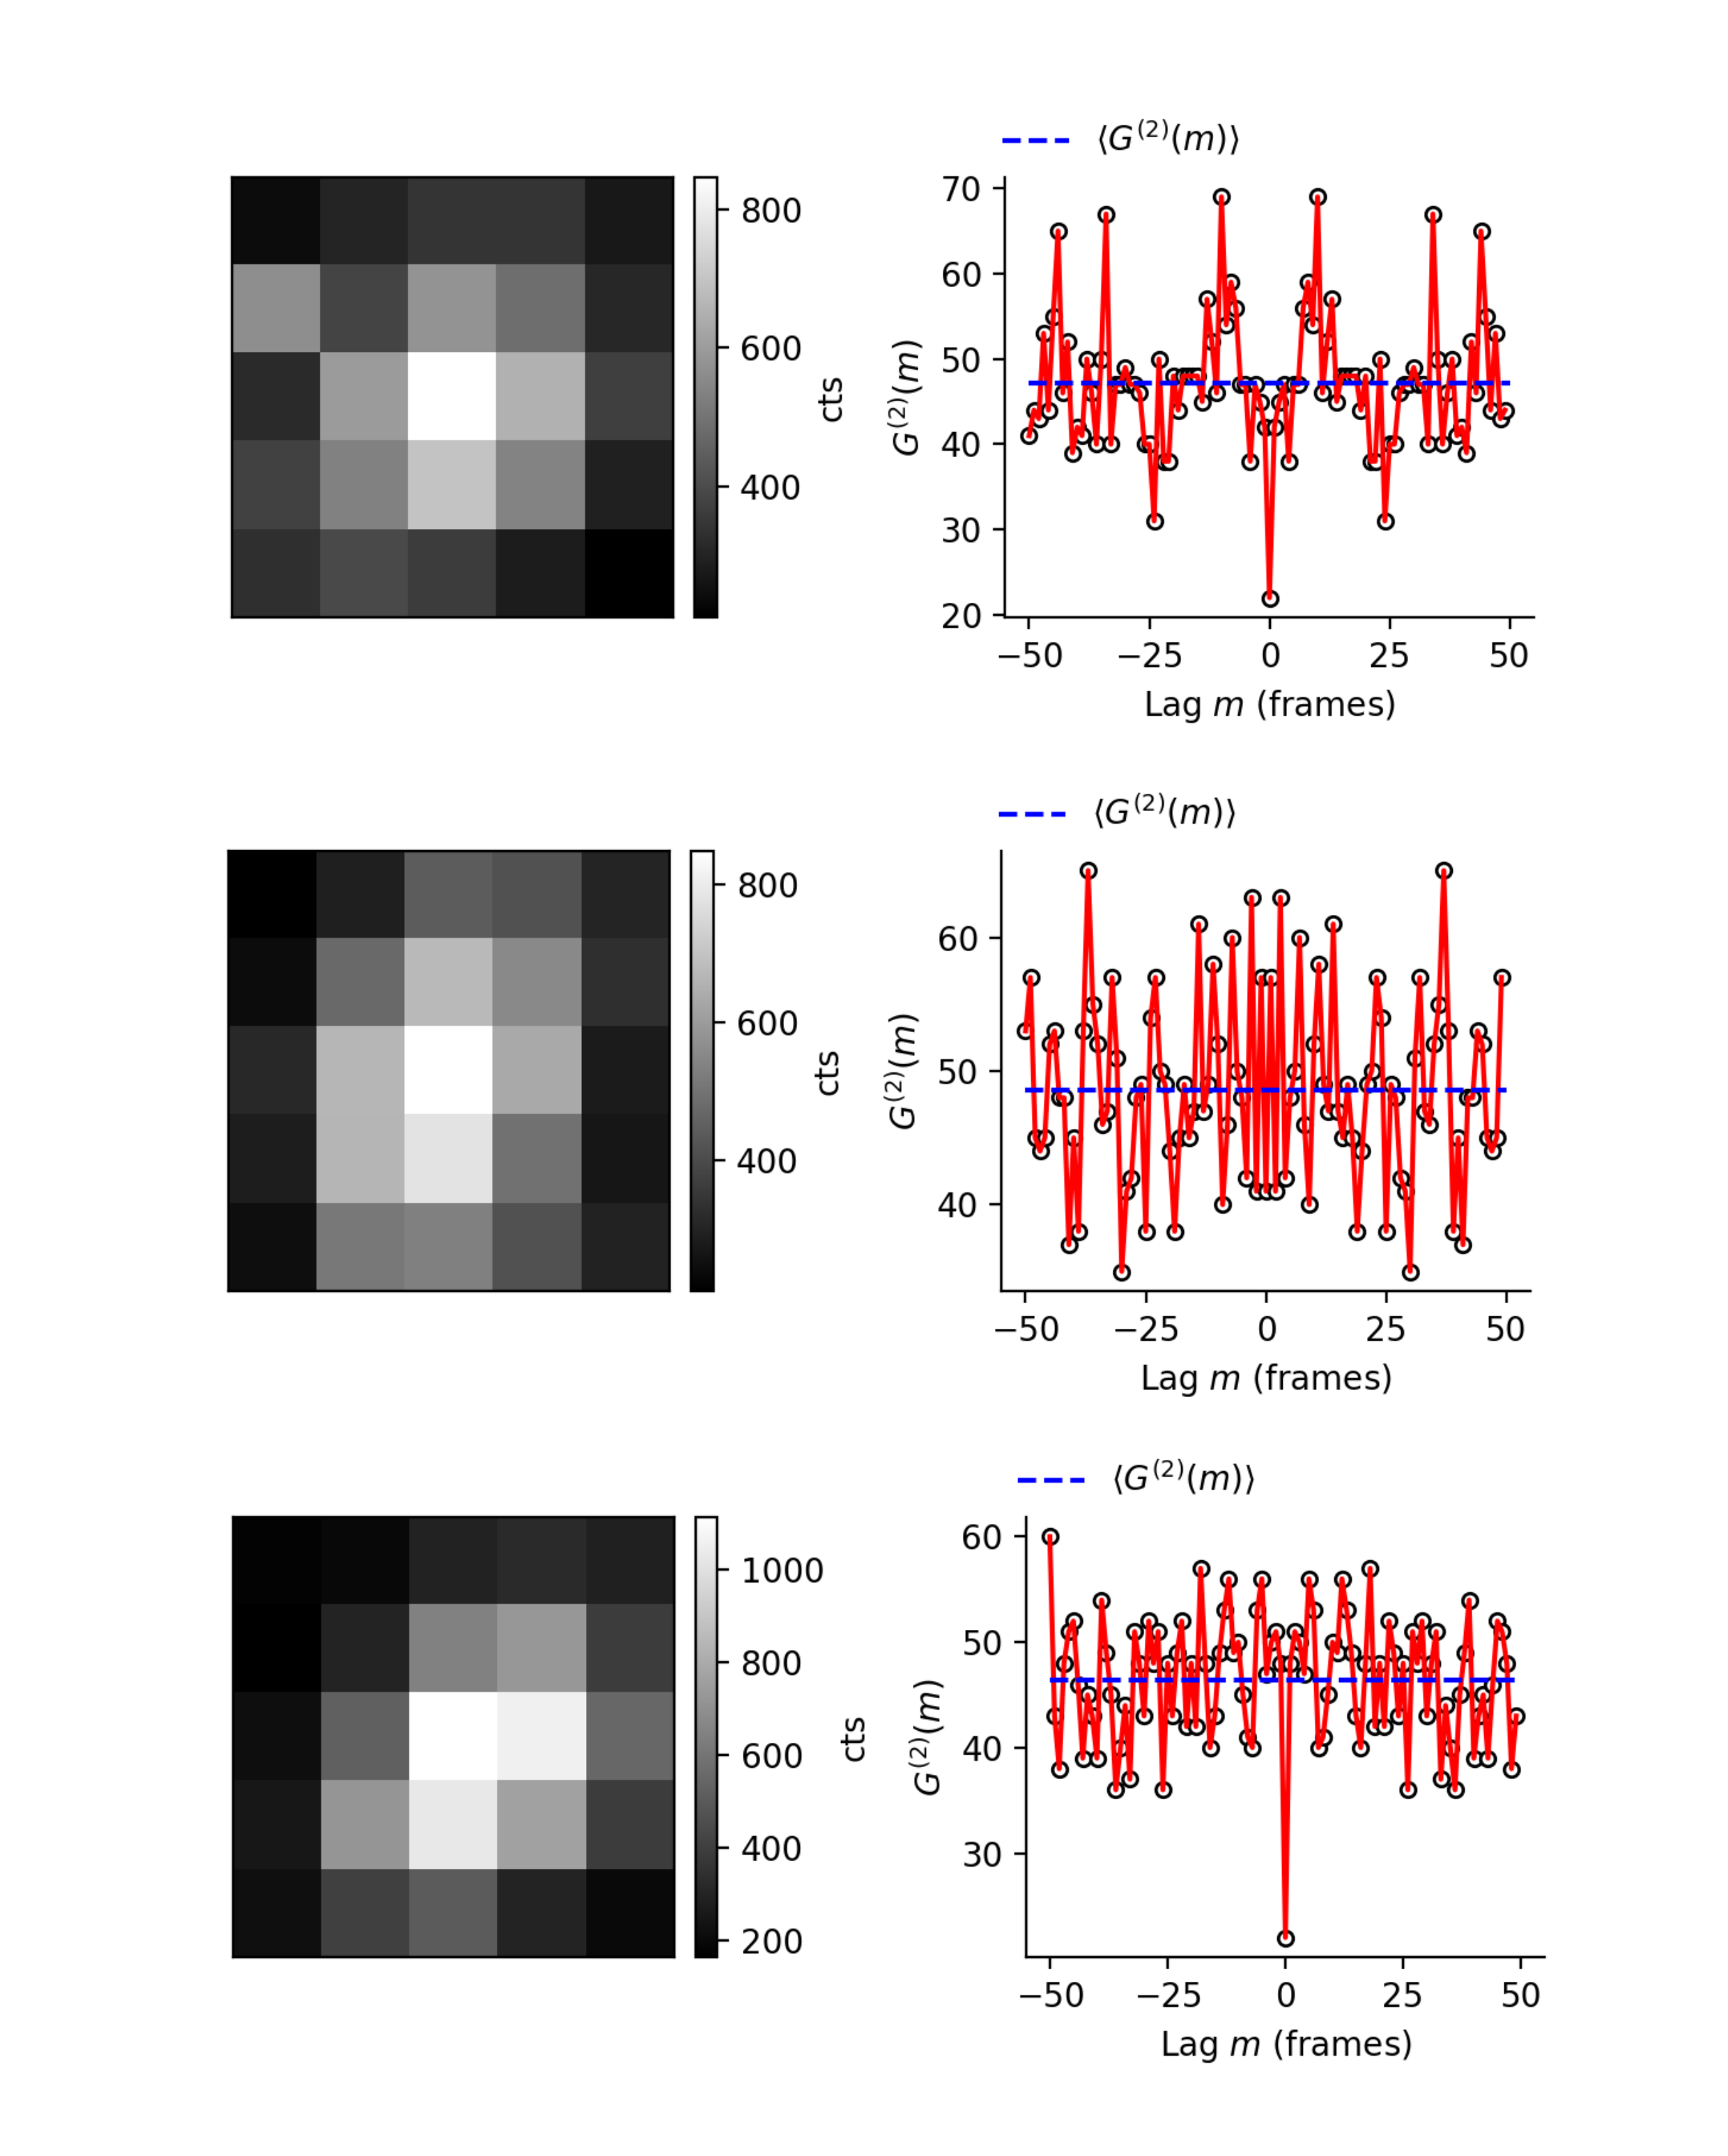
\includegraphics[width=14cm]{/Users/cwseitz/git/cwseitz.github.io/docs/phd/spad/spad/media/G2.png}
%\caption{\textbf{Example $G^{(2)}(m)$ functions}. Example quantum dot images and respective $G^{(2)}(m)$ functions, taken with 1us frames 500kHz laser repetition rate.}
%\label{fig:fig32}
%\end{figure*}    

\subsection{Discussion}

%Fluorescence intermittency can affect the observed photon-number fluctuations and could be expected to affect the value of $g^{(2)}(0)$ or the posterior on the number of active fluorescent emitters. However, the signal photon number per frame will follow Binomial statistics even in the presence of blinking, the only consequence of which is an effective reduction of the detection probability $\zeta$. If the effect of censoring photons by blinking and lowering the quantum yield can be accounted for, the technique used here may be compatible with common super-resolution techniques such as stochastic optical reconstruction microscopy (STORM). 

%The acquisition times necessary to obtain sufficient photon counts for computing the necessary statistics can potentially be very short. Most fluorophores have relaxation times in the nanosecond range and thus photons can be collected at a rate of at tens of millions of excitation pulses per second. These rates are currently difficult to obtain, however, due to limitations in triggering frequency and detector throughput. The SPAD camera used in this study has a minimum exposure time of 20 nanoseconds. Furthermore, the data volume can quickly become intractable due to the need for several thousands of frames for a millisecond-scale exposure time. This is currently a complication for techniques like STORM and advancements in the automation for data acquisitions are necessary. The speed of MCMC based localization remains a limitation for post-processing, and optimization of the processing time for localization is left for future work. 

%In conclusion, we propose a single molecule imaging technique that allows for counting of fluorescent molecules by modeling the quantum properties of fluorescence emission. The technique does not require a nonclassical light source and is designed to supplement standard single molecule localization microscopy techniques. The proposed method can be implemented with a standard widefield fluorescence microscope.

Here, we leveraged the recently developed SPAD array to spatially resolve the photon counting histogram with a widefield microscope. The PCH was integrated into a Bayesian inference scheme to extract the number of fluorescent emitters throughout the field of view and measure the second order coherence function. We demonstrated accurate counting of fluorescent quantum dots and fluorescent dyes bound to DNA origami, suggesting that this is a capable method for quantitative widefield fluorescent microscopy. Future work may assess more complex fluorescent imaging scenarios. 

For example, fluorescence intermittency or photobleaching leads to a $\zeta(t)$ which is not constant and can be fluorophore specific. This may affect the observed photon-number fluctuations and the PCH function $\mathcal{L}_{\mathrm{signal}}(n_{\mathrm{signal}})$ used here may no longer be stationary. Therefore, due to the unique dynamics of $\zeta(t)$ for each fluorophore, this PCH is no longer appropriate and one can expect more complex behavior of $g^{(2)}(0)$. As an example, challenges may arise in distinguishing one homogeneously emitting fluorophore and several blinking fluorophores. If the effect of censoring photons by blinking can be accounted for, the technique used here may be compatible with common nanoscopy methods which rely on fluorescence intermittency. However, neither of these effects need be considered here. The tested quantum dots are photostable and photobleaching of ATTO532 could be mitigated under the experimental conditions used. Moreover, the on and off state lifetime of tested quantum dots and are significantly longer than the acquisition sequence, making fluorescence intermittency negligible. 
 
The acquisition times necessary to obtain sufficient photon counts for computing the necessary statistics can potentially be very short. Most fluorophores have relaxation times in the nanosecond range and thus photons can be collected at a rate of tens of millions of excitation pulses per second. These rates are currently difficult to obtain, however, due to limitations in detector throughput. Moreover, the data volume can quickly become intractable due to the need for several thousands of frames for a millisecond-scale exposure time. 

Theoretical and experimental estimation of $g^{(2)}(0)$ demonstrate that the suitability of this measure can depend on experimental conditions. Collection of thousands of photons is necessary to reduce the error in the $g^{(2)}(0)$ value to its minimal value. Furthermore, we showed experimentally that low signal to background ratios results in loss of the binomial character of the data. This suggests the compatibility of bright fluorophores (such as quantum dots) for antibunching-based measurements. On the other hand, the Bayesian inference scheme of the fluorophore number will not be as sensitive to the fluorophore brightness in this way, as the PCH can effectively model various $\zeta$ values. 

Lastly, the method proposed here may lead to significant advances in localization microscopy. Many of these schemes utilize the concept of precise localization of fluorescent emitters to produce super-resolved images \parencite{Rust2006,Betzig2006}. However, an inherent problem with such methods is the assumption that fluorescent emitters are isolated, which can lead to undercounting and localization errors. Various models for multi-emitter localization have been developed to approach this issue statistically \parencite{Nehme2020,Speiser2021,Li2019,Fazel2019}, which necessarily treat the number of fluorescent emitters as an unknown. The approach proposed here provides a physical means to quantifying active fluorescent emitters based on widefield photon counting.

In conclusion, we propose a single molecule imaging technique that allows for counting of fluorescent molecules by modeling the quantum properties of fluorescence emission. The technique does not require a nonclassical light source and is designed to supplement standard single molecule localization microscopy techniques. The proposed method can be implemented with a standard widefield fluorescence microscope.

\clearpage
\begin{figure}
\centering
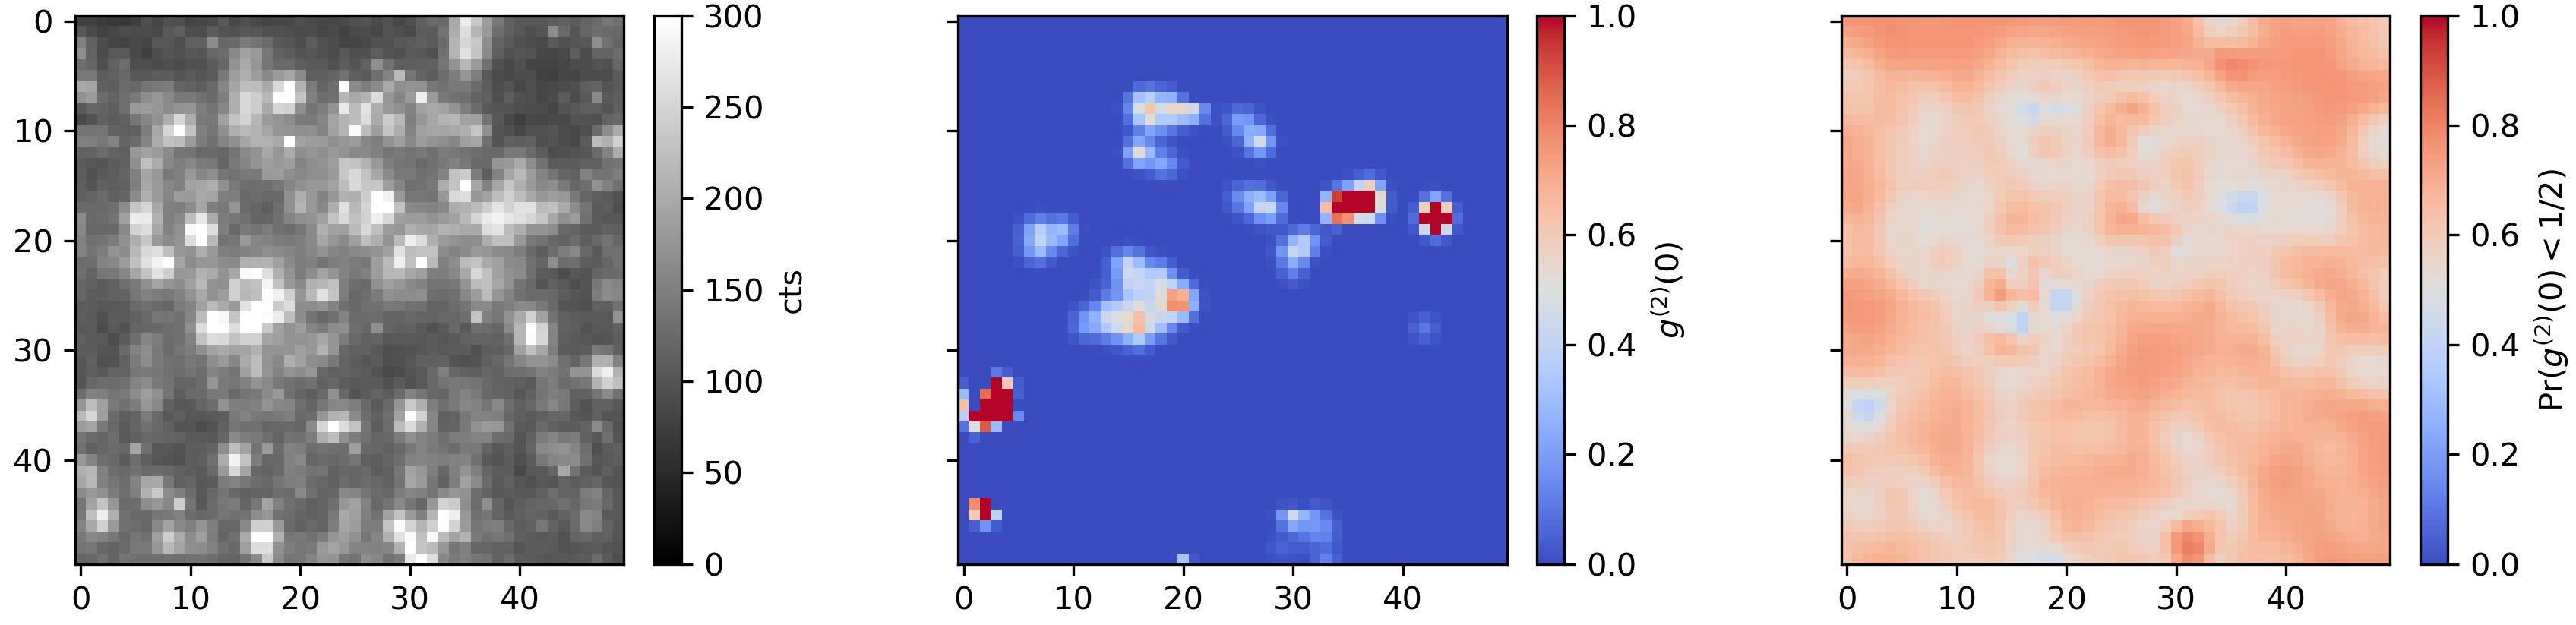
\includegraphics[width=16cm]{/Users/cwseitz/git/cwseitz.github.io/docs/phd/spad/spad/media/Figure-2.png}
\caption{\textbf{Theoretical scaling of the second-order coherence with the fluorophore number} (a) Expected number of coincidences at zero-lag (black) and the $g^{(2)}(0)$ ratio (red) in the case of pure binomial or pure Poisson photon statistics, as a function of the fluorophore number. Poisson and Binomial data are assumed to have an identical mean of 0.01 (b) $g^{(2)}(0)$ as a function of the fluorophore number for zero background conditions (pure binomial statistics) and various $\zeta$ values (c) $g^{(2)}(0)$ as a function of the fluorophore number for nonzero background conditions (Poisson-Binomial statistics, $\lambda=0.0075$) and various $\zeta$ values.}
\label{fig:binomvpoiss}
\end{figure}  


\begin{figure*}
\centering
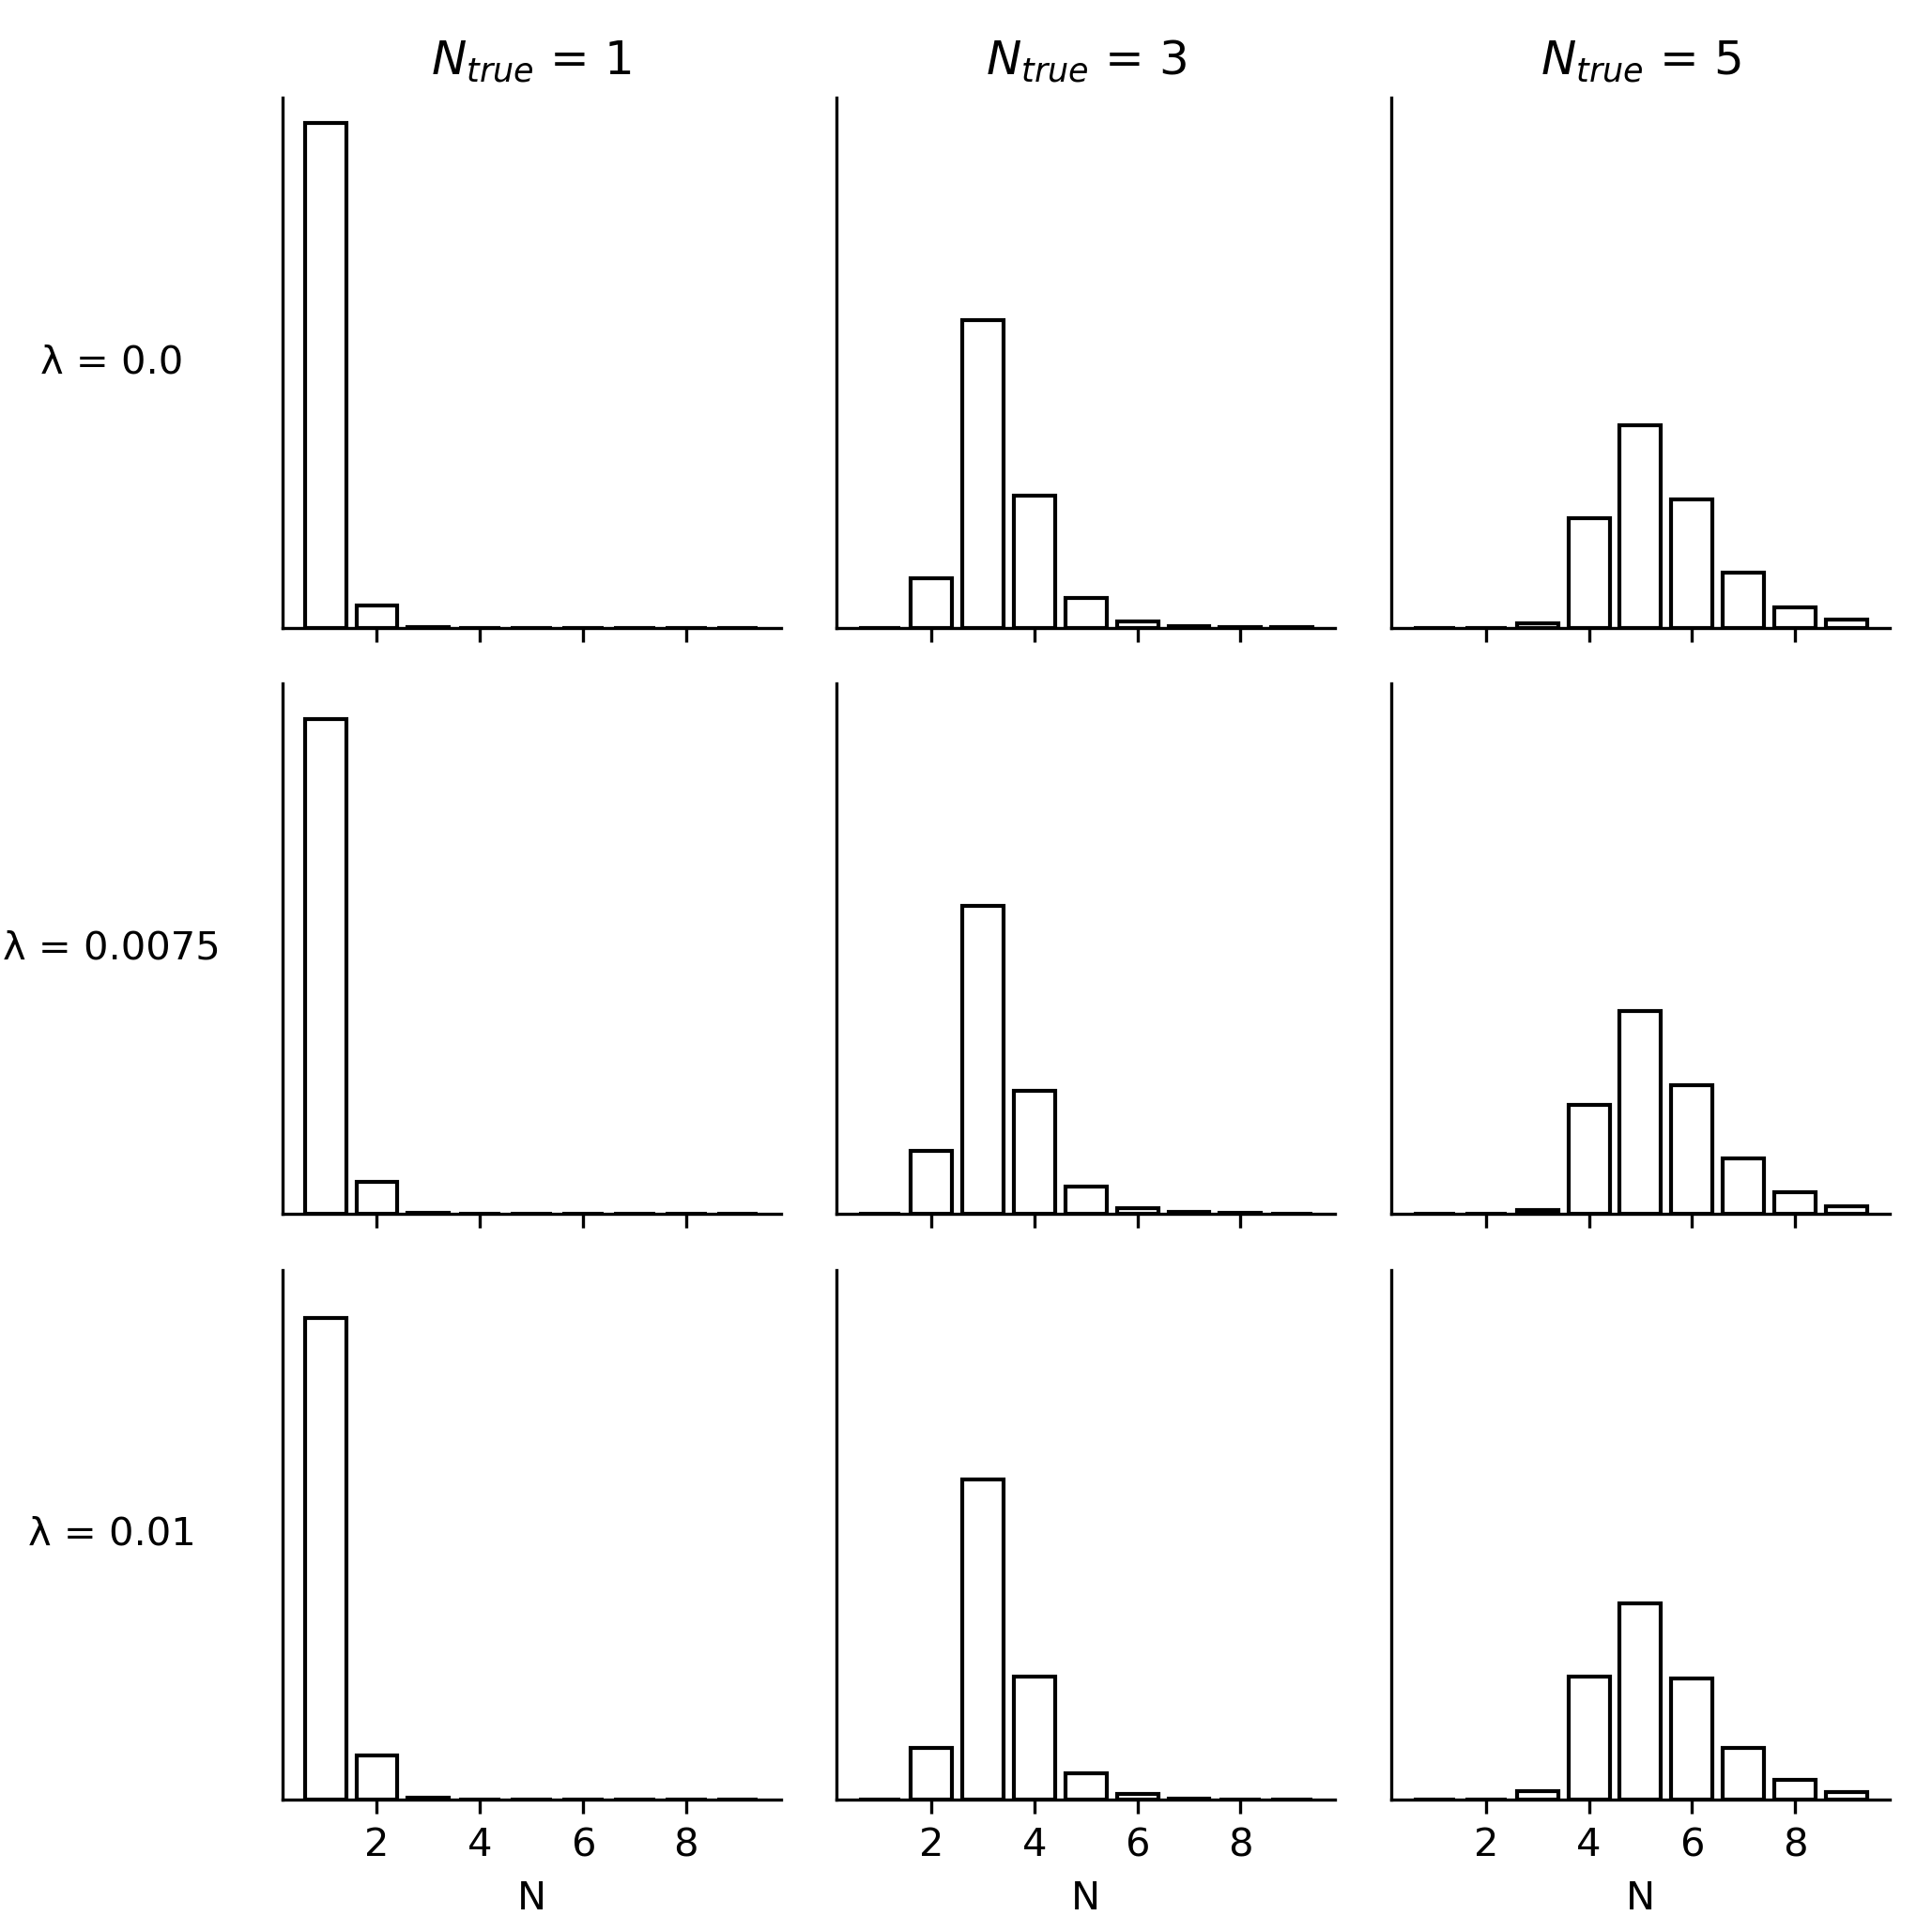
\includegraphics[width=14cm]{/Users/cwseitz/git/cwseitz.github.io/docs/phd/spad/spad/media/PoissonBinomialPost-1.png}
\caption{\textbf{Posterior distributions of the fluorophore number} Samples from the Poisson-Binomial convolution distribution using $\zeta=0.01$ for various values of $\lambda$ and $N=1,3,5$ were simulated. The variable $\zeta$ was integrated out by Monte Carlo integration, sampling 1000 $\zeta$ values from the prior distribution (see main text for details)}
\label{fig:fig9}
\end{figure*}    

\clearpage
\section{Future directions: quantum illumination strategies}

In recent years, novel quantum illumination strategies have leveraged spatial correlations between downconverted photon pairs to demonstrate the first quantum illumination full-field imaging protocol. These spatial quantum correlations are generated by a nonlinear optical process referred to as spontaneous parametric downconversion (SPDC). SPDC is typically realized using a nonlinear crystal such as Beta Barium Borate (BBO) or $\beta$-BaB$_2$O$_4$. BBO crystals are highly anisotropic and exhibit nonlinear optical properties, which means that polarization of the crystal varies nonlinearly with electric field strength. This nonlinear behavior can lead to a number of useful effects such as second harmonic generation, third harmonic generation, or SPDC \parencite{Boyd2020}. In the SPDC process, a pump photon typically in the ultraviolet range is downconverted into a pair of lower-energy photons, with wavelengths in the visible range. These photons are known as signal and idler photons. This process is a purely quantum mechanical one, and the daughter photons born in this process possess useful quantum mechanical properties. Indeed, physical principles such as conservation of energy and momentum require that the daughter photons born in this nonlinear process are spatially entangled in several degrees of freedom \parencite{Boyd2020}. 


A relatively straightforward application of SPDC is prediction of photon arrival times of the signal beam by measurement of the idler beam with a single photon sensitive detector. For example, this has been applied to improve the signal-to-noise ratio for measuring the absorption of objects through sub–shot-noise measurements \parencite{Brida2010} or imaging through detector noise and background signal \parencite{Gregory2020,Wolley2022}. In such applications, twin beams produced through the SPDC process are directed to different regions of a spatially resolved detector such as a CCD camera or single-photon avalanche diode (SPAD) array detector. By performing a pixel-by-pixel AND-operation between two regions of the array detector containing the SPDC beams, we can preferentially select correlated photon-pair events and reject uncorrelated background light and sensor noise events. Heralding photons using the signal and idler beams involves detecting one photon (either the signal or idler) and using this detection to infer the presence of its entangled counterpart. This method enhances the precision of photon detection and significantly improves the signal-to-noise ratio in quantum imaging.

This methodology has yet to be fully demonstrated in single molecule imaging or localization microscopy, which is generally quite sensitive to background signal or detector noise. Moreover, typical CCD	 technologies do not possess the time resolution of novel SPAD arrays, which may permit spatially resolved coincidence detection of photon pairs with nanosecond time resolution. Incorporating this technique into fluorescence imaging may further enhance the imaging quality and localization precision. By utilizing the known fluorescence lifetime of a single photon source such as a fluorescent dye molecule, one can possibly herald a fluorescence photon by measurement of the idler beam.

